\chapter{Case Studies}
\section{Analyzing the power market structures and business opportunities in select cases}

PJM: symmetric (self-schedule, pool-auction), obligation (load contributing factor), market-based, imbalance(enforcement, 10\% waved for VRE),

Germany: asymmetric (balancing energy market vs frequency control market), 

AEMO: asymmetric (AEMO pays for provider, charge regulation from either all generators or all consumers, and charge contingency from causer)

\label{sec:qualitative-analysis}
The super-set of I is the set of selected energy market segments in different geographies:

\begin{equation*}
I \subseteq  \begin{cases}
\{Day~Ahead, Real~Time\} & PJM \\
\{Day~Ahead, Intraday, Balancing\} & Germany \\
\{Real~Time\} & NSW
\end{cases}
\end{equation*}

The superset of I is the set of selected reserve market segments in different geographies:

\begin{equation*}
J \subseteq  \begin{cases}
\{RegA, RegD, SR, NSR, DASR\} & PJM \\
\{PCR, SCR+, SCR-, TCR+, TCR-\} & Germany \\
\{Lower, Raise\} \times \{REG, 6SEC, 60SEC, 5MIN\} & NSW
\end{cases}
\end{equation*}

\subsection{PJM}
\subsubsection{Organization of PJM power markets}
Marketplaces
Timeline

\subsubsection{Players}
A Load Serving Entity (LSE), as is defined officially by PJM, is "any entity that has been granted authority or has an obligation pursuant to state or local law, regulation, or franchise to sell electric energy to end-users that are located within the PJM RTO. An LSE may be a Market Buyer or a Market Seller"\cite{PJM2017b}. Therefore, LSEs refer to all market participates in PJM who have rights and obiligation to act in all the power marketplaces of PJM, including the energy, capacity and ancillary services markets. 

Curtailment Service Providers (CSPs) are members in PJM markets specializing in demand response. A CSP is an intermitted agency that provides the end-user DR to the wholesale market. \cite{PJM2017b} \cite{Wang2015} The role of the CSP is actually a legacy product from the liberalization of retail markets in PJM. Once the retail competition began, PJM allowed LSEs to provide DR not only for their own customer but also for customers of other LSEs. The role of the CSP was created to facilitate the liberalization and competition. \cite{PJMInterconnection2017}

\subsubsection{Balancing mechanism}
submit offer - rebid - update information up to 65 mins - deviation charged with real-time

reviewed the participation, violating -> suspend activity, enter enforcement

LSE obiligate to purchase (or self-schedule) reserve, obiligation as a proportion to its contributing flow to the grid. \cite{PJM2017c} This incents liquidity in the market with competitions on both buyer's and seller's side. However, the obiligation does not reflect their actual needs.\cite{Wartsila2014}

CSP
intermitted agency
allowed to voluntarily respond to the LMP

\subsubsection{PJM DR}

PJM DR is the umbrella for all distributed energy resources, including DR, behind-the-meter generations, storage, etc. since PJM does not specify how the load is reduced. However, PJM DR program does not allow energy injection beyond the meter and receive wholesale compensation.\cite{PJMInterconnection2017}. This issue is currently under discussion in Special Market Implementation Committee meetings.

DR emergency fast changing over years \cite{Brown2015}
Since the DR in the wholesale market as a supply recouse will cause double payment issue where a customer may receive wholesale energy revenue and retail cost savings for the same MW of load reduction, PJM states that DR participation in the retail market on the demand side would be more ideal. And they are discussing to revisit the mechanism. Therefore, this value is not fully modeled in our study.

LSE
buyer or seller in Energy, and reserve market

\subsubsection{Identify business model}

\subsubsection{Accounting}





The real-time market price is applied for all deviations from day-ahead planned schedule, including Regulation, Primary and Supplementary Reserves.

\begin{equation*}
\pi_t^{e,j} = \pi_t^{e,i} ~~~~ i \in \{Real~Time\}, j \in \{RegD, RegA, SR, NSR, DASR\}
\end{equation*}

The capacity prices of reserves are computed using a complex algorithm, taking into account a list of specifications of the resrouce, e.g. the performance \& historical performance, benefits factor, milleage, etc. The detailed calculations can be found in appendix. As outputs, we will get deterministic values for $j \in \{RegA, SR, NSR, DASR\}$, and the upper and lower bounds, $\overline{\pi}_t^{r,j}$ and $\underline{\pi}_t^{r,j}$, for $i \in \{RegD\}$.

%Reg = RMCCP + RMPCP + LOC
%LOC = 0
%RMCCP = 
%RMPCP = Milleage
%Effective MW = BF * MW
%BF is determined with the average and upper, lower bounds

\subsection{Germany}
$\pi_t^{e,i}, i \in \{Balancing\}$, is the the price for balancing energy (reBAP), which exist only in Germany

$\pi_t^{r,j}$ and $\pi_t^{e,j}$ are based on principle of pay-as-bid. The weighted-average values are available in the datasets.

%Market participants in Germany are organised into balancing groups, known as Bilanzkreise (BK). BK can range from individual large generators to aggregations of smaller renewable generations, to a Stadwerke representing large portions of aggregated demand.

%Every balancing group operator is responsible for following a planned schedule with a 15-minute resolution. Deviations from the planned schedule are balanced physically by the TSOs and settled financially with the BK. There is a legal obligation on Bilanzkreise to balance their positions to the best of their ability.

Prices for balacning energy are unified across TSOs and determined according to the  balancing energy price settlement system (BK6-12-024) developed by Federal Network Agency (FNA) as of 01/12/2012.

\begin{equation}
\label{eq:reBAP}
reBAP = \frac{\sum net imbalance energy cost}{\sum net imbalance energy volume}
\end{equation}

\subsection{Australia-New South Walse}
The unit prices of reserve products, $\pi_t^{r,j}$ and $\pi_t^{e,j}$, are not available in datasets published by AEMO. Only weekly summary for total payment and recovery are provided. Due to the limits of available data, we are only able to perform calculations of total potential revenues, rather than thorough studies as in the other two geopraphies.

\newpage

\section{Quantitative studies and results}
So far we have discussed qualitatively the existing and potential opportunities for flexibility managment in the three geographies, and screened the possible business cases. Further to that, it is necessary to perform quantitative analysis in order to understand:

\begin{itemize}
	\item \textbf{Market Size:} the potential value creation in the market for flexibility management solutions, subject to certain generic system dynamics but without respect to cost dyanamics of specific technologies
	\item \textbf{Profitability:} the metric to judge whether a specific technology is profitable or not to extract certain amount of value from current or future markets taking into account cost elements
\end{itemize}

Based on the methodology introduced in Chapter \ref{ch:methodology}, we performed experiments with consideration of constaints from both markets and technologies. All three markets discuess previously and two technologies, i.e. energy storage system (ESS) and Electric vehicle to grid (EV2G), were studied. 

Specifically, the ESS with a system dyanmic that is able to release and absorb energy can be deemed as a generic flexibility source. The revenue derived using ESSs can be viewed as a reference of the maximum market potential from flexibility managment. Meanwhile, with cost parameters of a typical battery energy storage system (BESS), we can analyze the profitability of BESSs with results involoving elements of costs. 

On the other hand, EV2G is served as a more peculiar example of technology, with additional case-specific constaints like the EV driving behaviors compared to a generic ESS. Maximum revenue from this technology shall be bounded by values derived from the generic ESS, but the profits may deviate significantly from values of BESSs, as their cost dynamics and business models could be distinct with other. Details are to be introduced later in this section.

Two types of works were carried out. We first examined the value of markets for flexibility management under current market conditions, i.e. based on historical observations without involving the market simulation module (Section \ref{sec:market-simulation}). This allows us to obtain some concrete numbers to establish a comprehensive understanding toward the value of flexibility management in nowadays' power markets. 

Thereafter, as markets evlove rapidly especially with the disruption of fast-growing renewable generations, a view toward future market development is also necessary. As a immature business, valuation of markets for flexibility management would be sensitively affected by various factors. The multi-dimentional variances and unpredictable changes on non-technical issues like market design and regulatory adjustments make it almost impossible to accurately forecast the market size and profits in the future. Nonetheless, understanding the impacts of some key factors would provide us valuable guidances on the directional movement of the market and thus offer viable references for technology vendors' decision makers.

\subsection{Data, paramters and valuation metrics}
The electricity market data including price and volume in each marketplaces correspond to the actual market data from January 1st 2016 to December 31st 2016. While general rules for accounting and data availability have been discussed in Section \ref{sec:qualitative-analysis}, detailed pre-processes and how they were fitted in as inputs of our valuation model can be found in Appendix \ref{sec:accounting-data-prepare}.

For cost determinations, we would first use figures based on the present market pricing level, and then make scenarios with reduced costs to find the break-even point if it is not yet profitable. According to the International Renewable Energy Agency (IRENA)\cite{IRENA2017}, the cost for battery energy storage systems was analyzed as proportional to their energy capacity, $\overline{s}$, and the energy cost coefficient, $C^s$, for state-of-the-art lithium-ion batteries were reported to be ca. $\$350/kWh$ in 2016. The replacement cost were based on actual price from Tesla\cite{Tesla1}, one of the leaders in battery and electric vehicle markets. The operating life is set to be 6000 FCEs, which corresponds to an optimistic estimation by Sandia National Laboratories\cite{Akhil2015}. Designed life time is assumed to be 10 years. Discount rate is made as 10\% as is discussed in Section \ref{sec:cost}. The technology costs were made to be zero so that the derived profits will be the margins that can be possibly realized by technology vendors. All the parameters for cost calculation are summarized in Table \ref{table:cost-parameters}. 

\begin{table}[h!]
	\begin{center}
		\begin{tabular}{ l  l  R{2.7cm} } %R{2.7cm} |}
			\hline
			\textbf{Items} & \textbf{Unit} & \textbf{Value} \\% & \textbf{Reduced Cost} \\
			%\hline
			\hline
			Energy cost coefficient, $C^s$ & $\$/kWh$ & 350 \\%& 140 \\
			%\hline
			Power cost coefficient, $C^r$ & $\$/kW$ & 0\\% & 0 \\
			%\hline
			Technology cos,t $C^0$ &$\$$ & 0\\% &0\\
			%\hline
			Replacement cost coefficient, $C^s$ &$ \$/kWh$ & 150\\% & 60 \\
			%\hline
			Designed life time & \textit{year} & 10\\% \multicolumn{2}{c|}{10}\\
			%\hline
			Operating life time & \textit{FCE} & 6000\\% \multicolumn{2}{c|}{6000}\\
			%\hline
			Discount rate &$\%$ & 10\\% \multicolumn{2}{c|}{10}\\
			\hline
		\end{tabular}
	\end{center}
	\caption{Parameters for cost calculation}\label{table:cost-parameters}
\end{table}

It is worthwhile to point out again that by using the parameters described above, the ESSs are virtually battery energy storage systems (BESSs). This fits the purpose of case studies. However, the conclusions on profitability are not portal for other types of ESS, but it does not mean the methodology loses its generality. The value of revenue would still be valid for other types of technology as long as they can have the same function of shuffling energy between time slots. Furthermore, by using different data as inputs, our model can be utilized for analysis of profitability of other energy storage systems with different cost dynamics. 

In terms of EV2G studies, we first determined the battery parameters of EVs.

\begin{itemize}
	\item EV charging rate is 10kW, corresponding to the guidance provided by Tesla\cite{Tesla2} and a typical home charging infrastructure with 50A current limit. 
	\item The battery energy capacity per EV of 75kWh is taken from one of the most popular EV models\cite{Tesla3}.
\end{itemize}

Simulations are then performed to get EV driving profiles, which are based upon data from the California Department of Transportation's California Household Travel Survey for 2010-2012\cite{NREL_TSDC}. This survey carried out multiple objectives and included 79011 vehicles. For our work we focus on a proportion of the vehicles, 2910, which were fitted with GPS. These vehicles were monitored continuously for a 7-day window with the 1-second resolution. The GPS data is then processed into trip profiles, while include information of the location of each EV at each time step as well as the trips made by each EV. Furthermore, together with the parameters of the EV model we have selected above we simulated the SoC time series of the EV batteries. Finally, from the simulated results, we can statistically derive the value of probability distribution of EV plug-in $n^+$, plug-out $n^-$, and average state-of-charge (SoC) of batteries plug-in $s^+$, plug-out $s^-$, as introduced in Section \ref{sec:tech-simulation-module}. The results are shown as Figure \ref{fig:data-ev-number}-\ref{fig:data-soc} where we can see clear periodic patterns that are different between weekdays and weekends.

\begin{figure}[h!]
	\centering
	\centering
	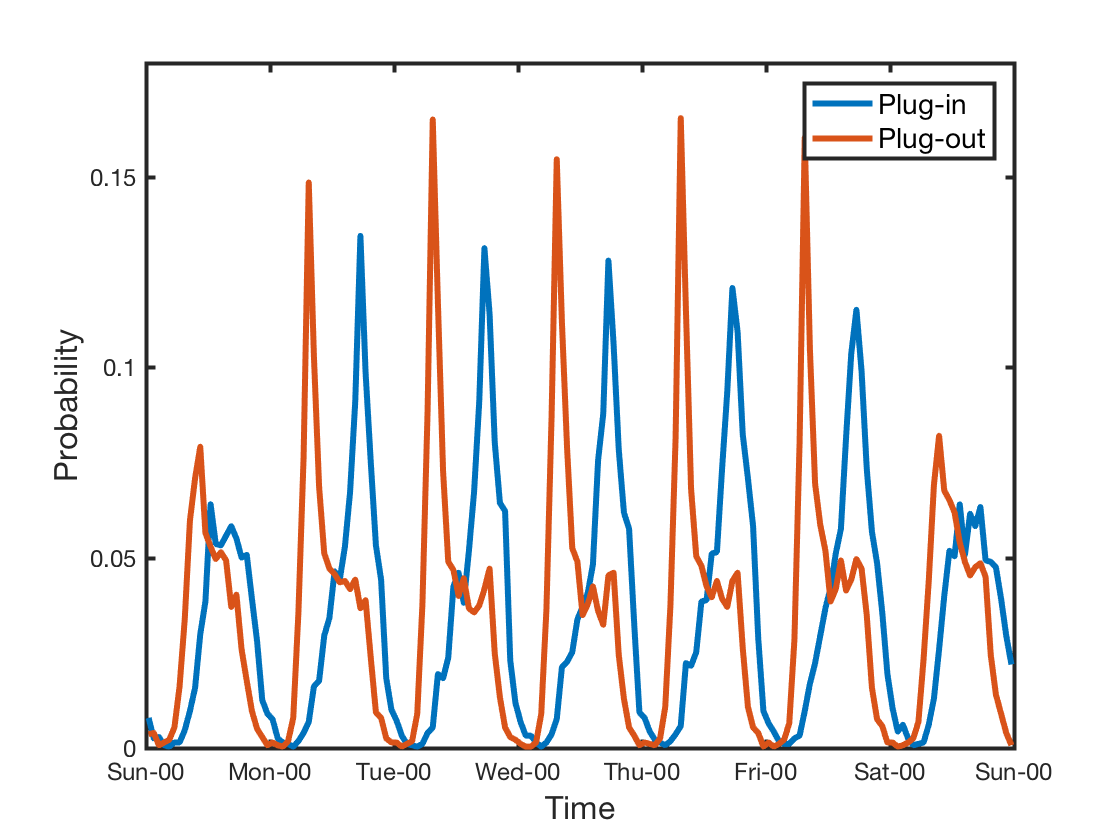
\includegraphics[width=0.8\linewidth]{Figures/Data_EV_number}
	\caption{Probability of EV plug-in/ plug-out}
	\label{fig:data-ev-number}
\end{figure}

\begin{figure}[h!]
	\centering
	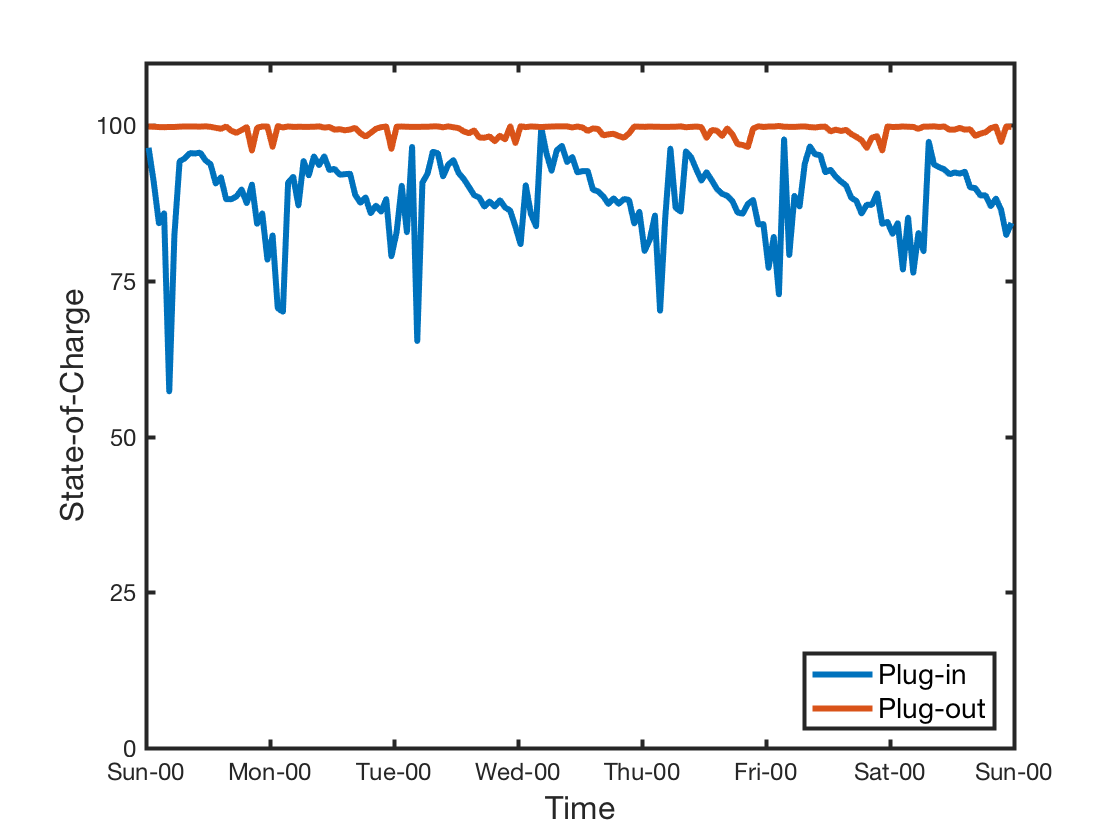
\includegraphics[width=0.8\linewidth]{Figures/Data_SoC}
	\caption{Average SoC of EV when plug-in/ plug-out}
	\label{fig:data-soc}
\end{figure}

The metrics to evaluate the system performance are slightly different between ESS and EV2G. For ESS, the criteria in the evaluation metrics include
\begin{itemize}
	\item \textbf{Revenue:} the total explicit revenue from electricity markets calculated as Equation \eqref{eq:module-revenue}, per annum
	\item \textbf{Operating Profit}: the total revenue net of operation-dependent costs (degradation cost), per annum
	\item \textbf{Profit:} the total revenue net of both operation-dependent and fixed costs, per annum
\end{itemize}

For EV2G, the fixed cost that is mainly related to procuring the battery stocks shall not be considered for a technology vendor. Furthermore, the implicit charging cost to compensate the energy consumed by EV driving are listed separately. Depending on the specific business model in practice, a portion of the implicit charging cost may be recovered by the technology vendors from the end-users, although in this thesis we did not exclude it from calculating the profit. As a result, the criteria are altered as:
\begin{itemize}
	\item \textbf{Revenue:} the total explicit revenue from electricity markets calculated as Equation \eqref{eq:module-revenue}, per annum
	\item \textbf{Implicit Charging Cost}: the cost of energy compensation for EV driving demands, calculated as the total energy consumption multiplied by average price over the span of one operational cycle, per annum
	\item \textbf{Profit:}: revenue net of costs including the implicit charging cost and battery degradation. The investments on technology are made to be zero as is discussed at the beginning of this section, per annum
\end{itemize}

As a result, the profit of a EV2G system is closed to the concept of operating profits for a ESS, which excludes the investment of procuring batteries. This implies two disparate business models. Cautions shall be raised while comparisons between these two technologies are made.

In order to determine the profitability and market size of ESS, we evaluated the system performance with different total sizes. Thereafter, we would select some key states in order to extract the most informative indicators to technology vendors. Overall, 4 scenarios would be analyzed and are illustrated by Figure \ref{fig:scenario-illustration} using an example with typical curve shapes. This example shows the results for a case of making arbitrage in day-ahead, real time energy markets and simultaneous delivering regulation services in PJM electricity markets. 
\begin{figure}[h!]
	\centering
	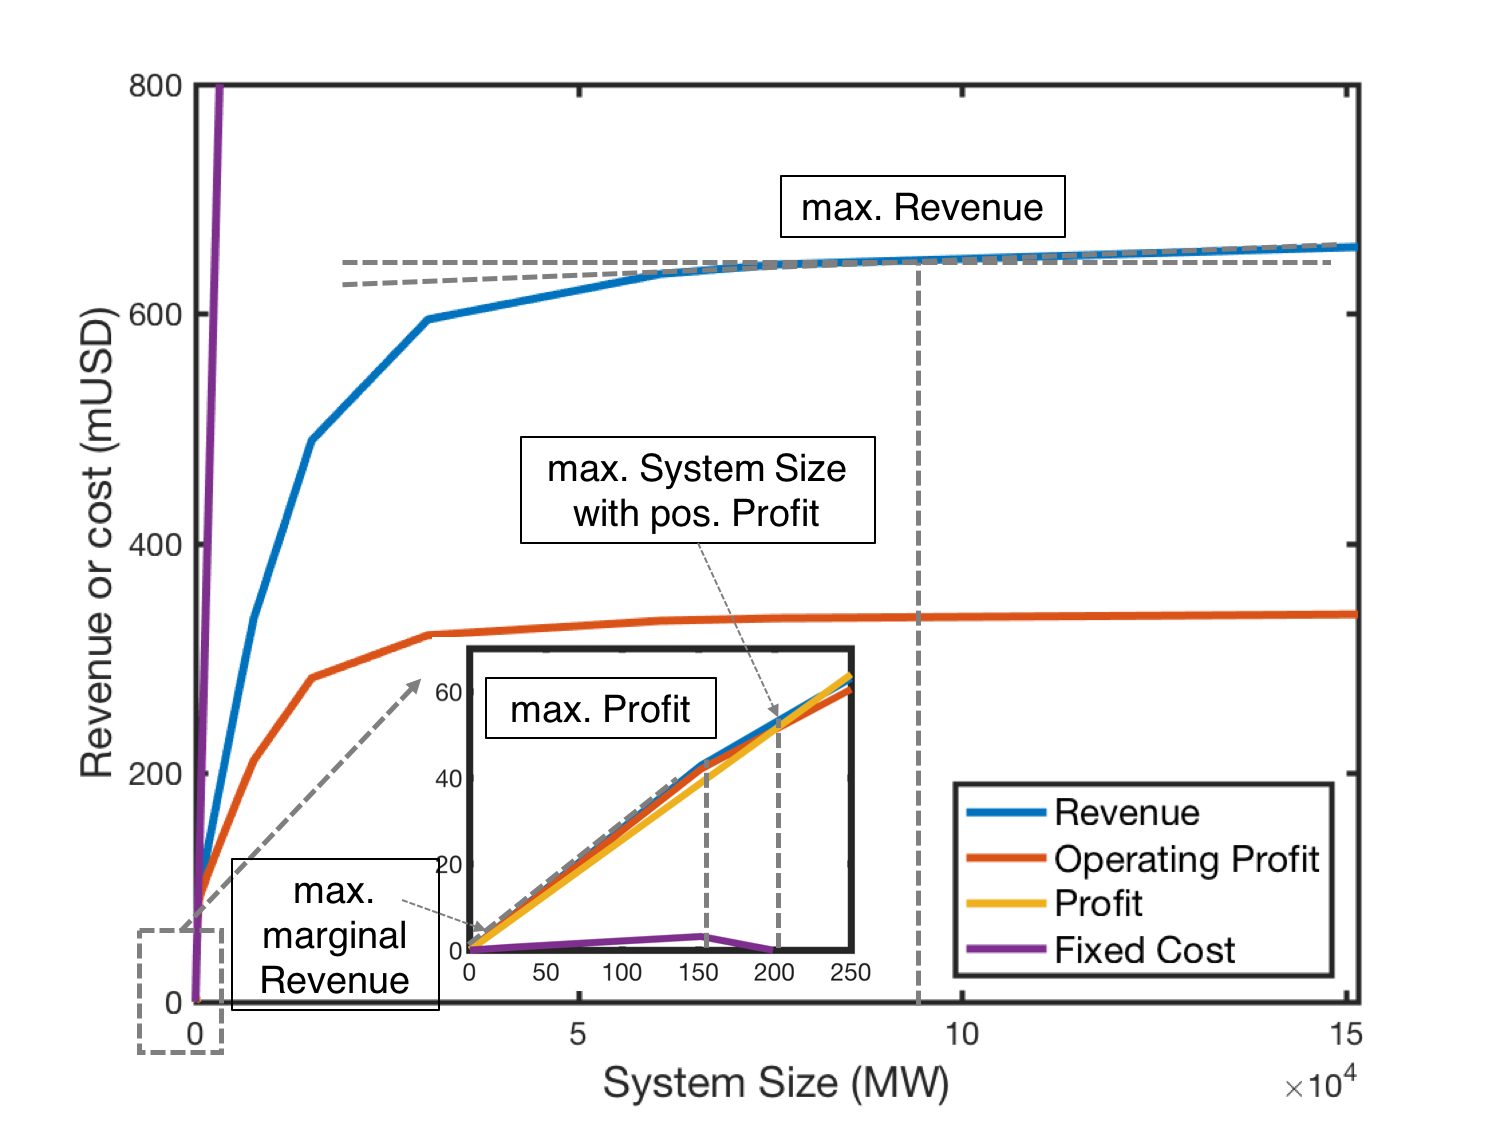
\includegraphics[width=0.95\linewidth]{Figures/Scenario_illustration}
	\caption{Graphic illustration of 4 scenarios}
	\label{fig:scenario-illustration}
\end{figure}

Two the most crucial states are:

\begin{itemize}
	\item ``\textbf{max. Revenue}": the state where the maximum potential revenue is extracted from the markets. The ``max. Revenue" state is determined as when the marginal increment of revenue is less than 5\% with additional system capacity, i.e. 
	\begin{equation*}
	\frac{\Delta\text{Revenue}}{\Delta\text{System Size}} < 0.05
	\end{equation*}
	Since in our studies, we found the operating profits are always in line with revenue, so this state is equivalent to``\textbf{max. Operating Profit}".
	
	The value of revenue in this scenario can present a reference of maximum market potential, i.e. maximum amount of revenue can be possibly realized, without respect to the costs. Profits tend to be negative in this scenario with inflated system size. However, it could still provide informative indicators to technology vendors as they might be able to develop technologies with lower costs than what we calculated in the case studies. 
	
	\item ``\textbf{max. marginal Revenue}": the state where the marginal incremental revenue is maximized.
	
	Since in our study, we found the operating costs were always in line with the revenue while the fixed cost were proportional to the system size. As a consequence, this state is always achieved with the smallest ESS size simulated when the market constraints are rarely activated.
	
	This state indicates the maximum potential return per unit system so reveals the profitability at the most optimistic condition. In order to make results be understood more intuitively, we would normalize the values in this scenario to be per unit system size. 
\end{itemize}

In addition, if the profit was found to be positive in the scenario of ``max. marginal Revenue", there are two more states that are worthwhile to draw attention to:

\begin{itemize}
	\item ``\textbf{max. System Size with pos. Profit}": the state indicating maximum possible system size where the profit is barely above zero. Since in our studies the profit either drops monotonically or decreases after an initial rise, this state is obtained when the profit falls to be 0.
	
	This scenario would inform technology vendors about when the market would be saturated. Without revolutionary innovations on technologies or drastic changes on market conditions, expanding the flexibility fleet beyond this scenario is likely to create losses rather profits. 
	
	\item ``\textbf{max. Profit}": the state where the profit is maximized.
	
	If the total system size goes beyond this scenario, it indicates that the competition will intensify and the profit will drop with additional market entrants.
	
\end{itemize}

These two scenarios would not exist if the profit in the scenario of ``max. marginal Revenue" is negative as it means the marginal revenue and marginal operating profits would never exceed the marginal fixed cost that is constant. 

Overall, ``max. marginal Revenue" indicates the potential market size, and the rest three scenarios illustrates the profitability and profitable market size with the pre-defined cost paramters.

In terms of EV2G, the size of the system (number of EVs) are not strongly related to the profitability of EV2G, if at all. Therefore, it makes no sense to analyze the optimal system size in relation to the profitability. Instead, we would show the market values under certain scenarios where the number of EVs is determined externally. 

\begin{table}[h!]
	\centering
	\begin{tabular}{ L{2.5cm}  R{4cm}  R{3.5cm} }
		\hline
		\textbf{Geography} &\textbf{Consumption (MW)} & \textbf{MP} \\
		%\hline
		\hline
		Germany & \num{59138} & \num{51869730}\\
		PJM & \num{87793} & \num{30331401}\\
		NSW & \num{7978} & \num{3364428}\\
		\hline
	\end{tabular}
	\caption{The metrics of scaling the market by average comsumption rate and metering points}\label{tab:MP}
\end{table}

Finally, we would normalize results with respect to the overall scale of the market, in order to make cross-regional comparison more intuitive. The main metric to represent the scale is the average consumption rate (in MW) in the whole market. Consequently, values of cash flows would be shown in unit of million USD per year per MW consumed (USD/$(\text{a} \cdot \text{MW})$). Meanwhile, the metering point (MP) is taken as a auxiliary metric and would be mentioned in certain circumstances as it represents the number of end-consumers in a market. The average consumption rates were obtained from the power markets data in 2016 and the statistics of MP are provided by commercial market data provider, Northeast Group\cite{NortheastGroup2016}\cite{NortheastGroup2017}\cite{NortheastGroup2017a}. All the relevant numbers are listed in Table \ref{tab:MP}.

The currency exchange rates are determined as the real market data as of January 1st 2018, when 1 EUR is equal to 1.20 USD and 1 AUD is equal to 0.78 USD\cite{Bloomberg}.

\subsection{Value of markets under current market conditions}
This section presents the results using historical market data. Since two types of technologies and markets in three geographies were studied, there are a total of six distinct setups with each comprises serveral use-cases. In addition, we included a cost break-even analysis specifically for ESSs as few profitable opportunities were found due to high costs on battery stocks.

\subsubsection{ESS in Germany: opportunities hidden by adverse market design of balancing energy and frequency control}

\begin{figure}[h!]
	\centering
	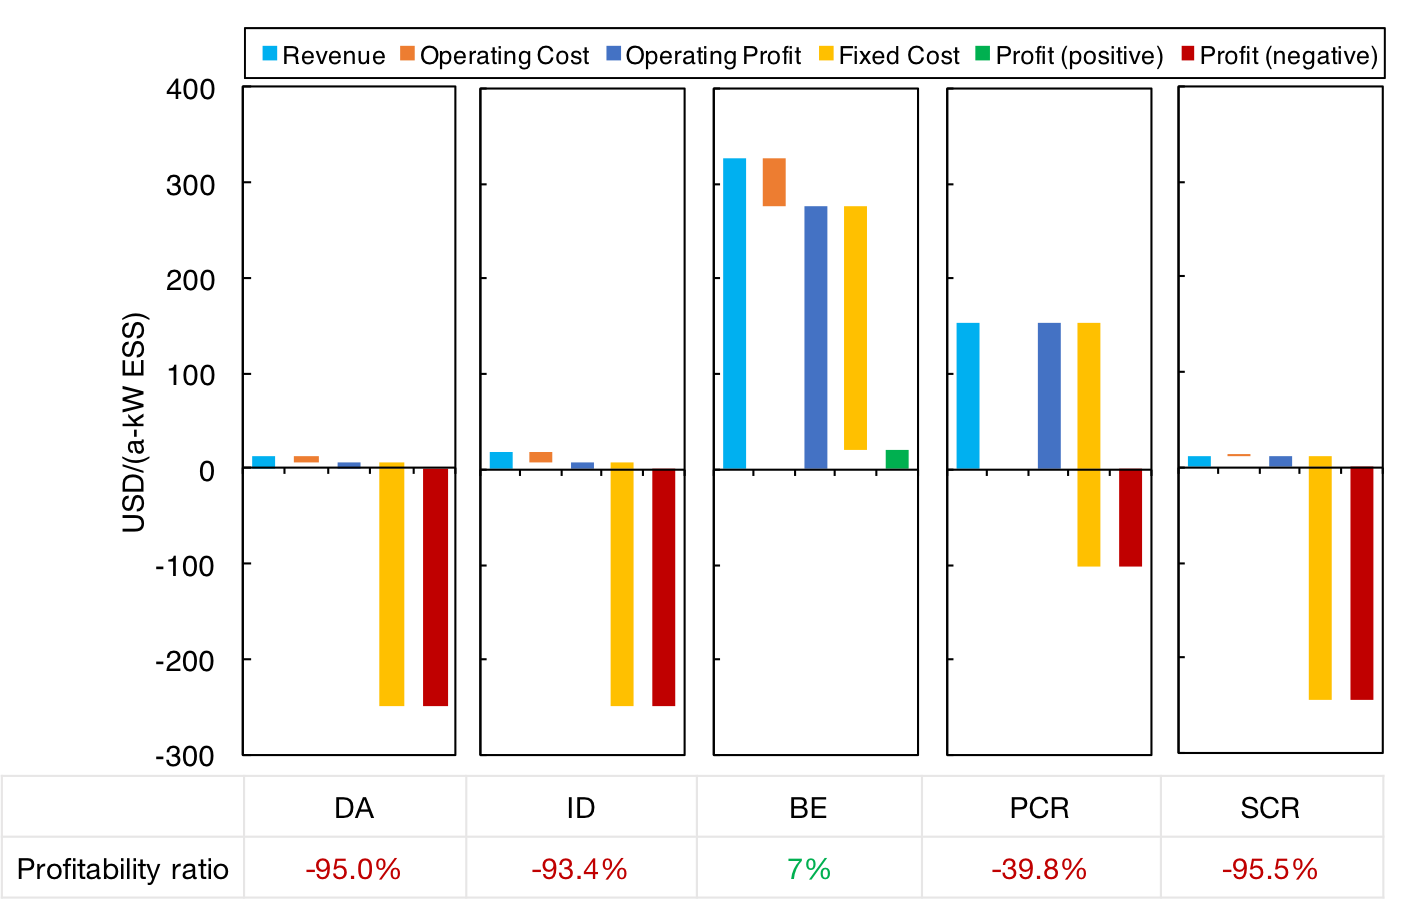
\includegraphics[width=0.9\linewidth]{Figures/Germany_ESS_profitability}
	\caption{Profitability of ESS in Germany electricity markets in the scenario of ``max. marginal Revenue"}
	\label{fig:germany-ess-profitability}
\end{figure}

\begin{figure}[h!]
	\centering
	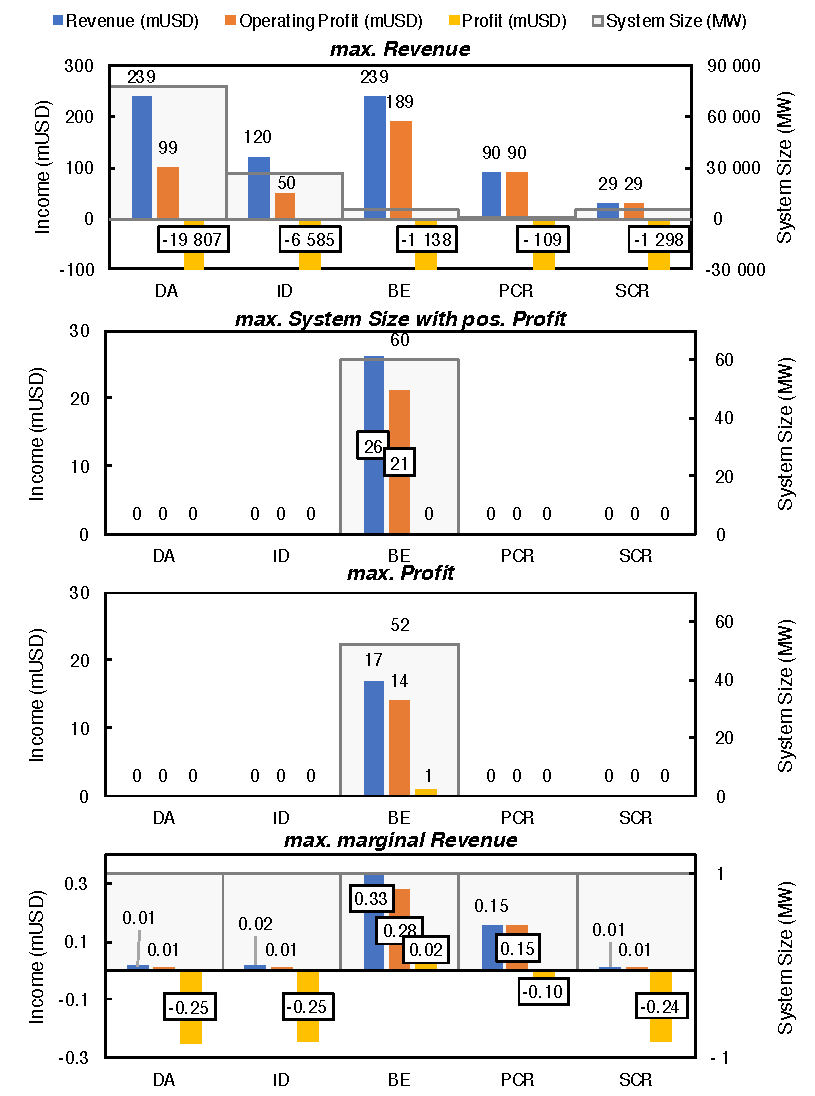
\includegraphics[width=0.9\linewidth]{Figures/Germany_ESS}
	\caption{Market size of ESS in Germany electricity markets in the scenario of ``max. Revenue"}
	\label{fig:germany-ess}
\end{figure}

As is discussed, profitability analysis can be performed using the scenario ``max. marginal Revenue", the results of which are depicted by Figure \ref{fig:germany-ess-profitability}. By showing values per unit ESS system installed, we can see the maximum unit return of ESS in Germany power markets. 

Meanwhile, with ample size of ESS, maximum potential market sizes can be derived, corresponding to the scenario ``max. Revenue".
Summarized by Figure \ref{fig:germany-ess}, annual cash flows are shown per MW consumption as normilzed values to the overal average consumption, \num{59138} MW . For example, the normalized revenue for arbitrage in day-ahead market is \num{4041} USD per year per MW consumption, which indicates the achievable revenue for a power system in Germay with 1 MW average load and corresponds to 239 mUSD/a in whole German market by mutiplying the base of \num{59138} MW.

It was found that the only profitable case is delivering balancing energy. As is analyzed in Section \ref{sec:qualitative-analysis}, this case corresponds to the situation of self-balancing where the players turn to the flexibility resource in avoidance of charges by TSOs for their imbalances. We further analyzed the maximum profitable system size and maximum profit of using the pre-defined BESSs; see Figure \ref{fig:germany-ess-profitable-size}.

\begin{figure}[h!]
	\centering
	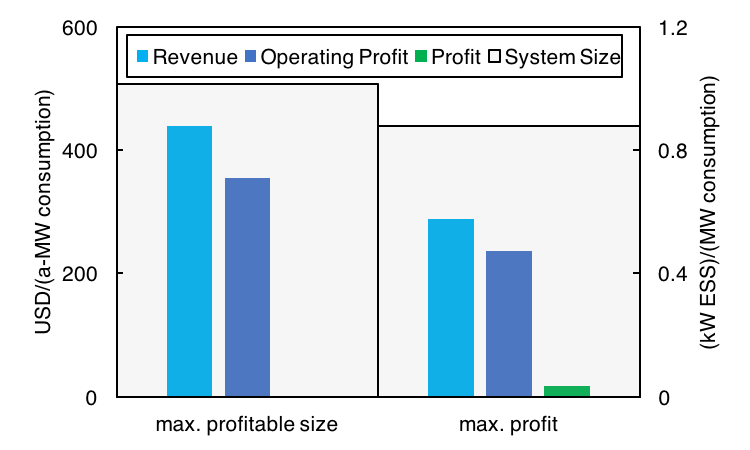
\includegraphics[width=0.9\linewidth]{Figures/Germany_ESS_profitable_size}
	\caption{Market size of ESS in Germany electricity markets in the scenario of ``max. System size with pos. Profit" and ``max. Profit"}
	\label{fig:germany-ess-profitable-size}
\end{figure}

It can be seen from Figure \ref{fig:germany-ess-profitable-size}, if being operated optimally BESSs with a size of up to 1 kW/(MW consumption) can generate profits by serving balancing energy, corresponding to a total 60MW in Germany. Nevertheless, it is challenging to be realized in practice. Market players do not have the right information to optimize their operational plans, since the balancing energy price, reBAP, is calculated \textit{ex-post} and highly volatile, hardly predictable, as is discussed in Section \ref{sec:qualitative-analysis}. On the contrary, if a system is designed to have ample size and tackle almost all imbalance events, it corresponds to a situation as the ``max. Revenue" scenario where we see negative profits from Figure \ref{fig:germany-ess-profitability}.

On the other hand, we noticed from Figure \ref{fig:germany-ess-profitability} that selling frequency control services to TSOs is less economically viable than using BESSs for self-balancing.The maximum marginal revenue from self-balance is significantly higher (33 times) than from selling frequency control products, while ideally the situation shall be reversed. The balancing energy charges are designed to recover the costs of activating frequency control services (calling for energy delivery) while the costs paid for securing capacity commitment are socialized, as have been fully discussed in Section \ref{sec:qualitative-analysis}. Theoretically, players shall get higher turnover in the frequency control markets than avoided balancing energy charges. Furthermore, the actual total payment for SCR in Germany is 176 mUSD in 2016 which is equavilent to \num{2976} USD/$(\text{a} \cdot \text{MW})$, while the maximum achievable revenue with BESSs are bounded at \num{490} USD/$(\text{a} \cdot \text{MW})$ as shown in Figure \ref{fig:germany-ess} with the rest 83.5\% of the market is intangible for BESSs . Our results imply that the current design of frequency control markets is neither economically efficient nor technically feasible to integrate the emerging BESS resources, which verifies our analysis in Section \ref{sec:qualitative-analysis}. We have argued that hurdles exist against emerging BESS to participate in frequency control markets with the non-energy-neutral signals and block-wise offering, especially for SCRs which demand significantly higher energy delivery than PCRs.

Facing either lack of information transparency in balancing energy charges or unfavorable market rules in frequency control markets, BESS players have no feasible options in the current market setup to make profits.

However, we may argue this situation shall not be long-lasting. We have already seen that certain amount of BESS will be a cheaper option to defer the expense on imbalance settlements compared to what are currently incurred. The market operators shall develop well-designed frameworks to encourage the participation of these resources that are beneficial to lower the overall system costs. In reality, there are indeed debates proposing possible solutions on this issue, e.g. letting TSOs who have the most abundance of information own and dispatch the storage resources\cite{He2012}, re-engineering the pricing mechanism of balancing energy\cite{Wartsila2014} and implementing favorable frequency control products for storage\cite{Megel2017}, etc.

As an implication for technology vendors, these possible movements on market designs shall be taken care of as it could suddenly turn over the feasibly profitability of using BESSs for balancing services.

Regarding arbitrages value in energy market, although the potential revenues are \num{4041} USD/$(\text{a} \cdot \text{MW})$ in day-ahead and \num{2029} USD/$(\text{a} \cdot \text{MW})$ in intra-day market, the losses would be incredibly high in order to materialize the revenue using BESSs; see Figure \ref{fig:germany-ess}. Even in the scenario of maximum unit return, the losses are about 10-20 times of the revenue; see Figure \ref{fig:germany-ess-profitability}. It is clear that the heavy investments on batteries cannot be recovered from making arbitrage in energy market. However, since the operating profits are always positive, if technology vendors can enable similar functions as BESS using technologies with smaller capital costs such as certain types of DR, it is still possible to make profits out of the market worth a total of over 300 mUSD per annum in Germany.

\begin{figure}[h!]
	\centering
	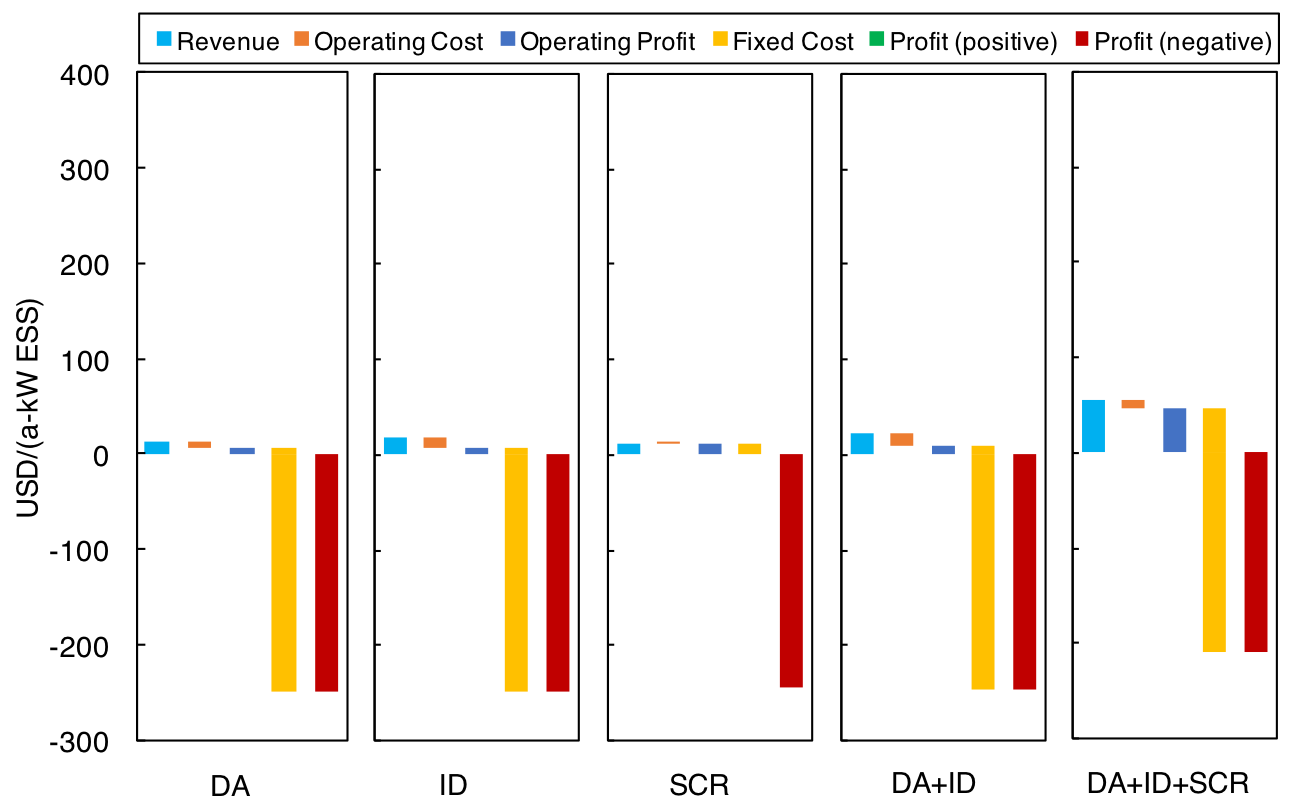
\includegraphics[width=0.95\linewidth]{Figures/Germany_ESS_profitability_multitasking}
	\caption{Profitability of ESS with multitasking in Germany electricity markets}
	\label{fig:germany-ess-multitasking-profitability}
\end{figure}

\begin{figure}[h!]
	\centering
	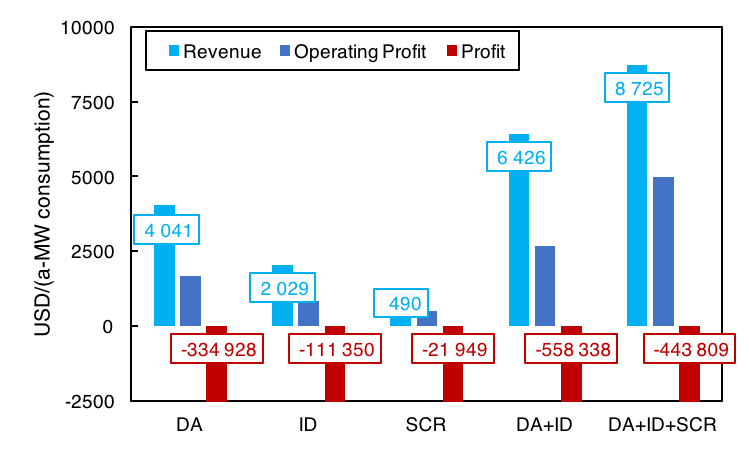
\includegraphics[width=0.95\linewidth]{Figures/Germany_ESS_multitasking}
	\caption{Market size of ESS with multitasking in Germany electricity markets}
	\label{fig:germany-ess-multitasking}
\end{figure}

As has been discussed qualitatively, in order to increase the profitability and find a way to neutralize the frequency control signals, we may stack operations in day-ahead, intra-day and secondary control reserve for multitasking. Figure \ref{fig:germany-ess-multitasking} shows the effects of multitasking.

While there are no significant synergies observed between day-ahead and intra-day markets (the unit returns remain unchanged in the scenario of maximum marginal revenue), stacking secondary control reserve with these two energy marketplaces will significantly improve the unit revenue (from 11 and 22 USD/$(\text{a} \cdot \text{MW})$ to 54 USD/$(\text{a} \cdot \text{MW})$) as well as the maximum revenue potential (from \num{6426} USD/$(\text{a} \cdot \text{MW})$ plus \num{490} USD/$(\text{a} \cdot \text{MW})$ to \num{8725} USD/$(\text{a} \cdot \text{MW})$). The maximum unit operating profit, as a consequence, raises by 4.5 times. The increment of maximum potential revenue of \num{2299} USD/$(\text{a} \cdot \text{MW})$ by stacking SCR on DA+ID indicates an additional revenue of \num{1809} USD/$(\text{a} \cdot \text{MW})$ are accessible for ESS in the SCR markets, reducing the intangible part from 83.5\% to 22.7\%. This corresponds to our previous analysis that the non-energy-neutral signal is indeed an issue for BESSs and has to be neutralized externally. Nonetheless, coping with third-party energy transactions requires the BESSs spare certain capacity to receive or release the energy, which reduces their availability in delivering SCR services. This is reflected on the result that this case with multitasking is still not profitable.

To sum up, while arbitrage is mainly constrained by costs on the technology side, making profits from balancing services is limited by adverse market frameworks although it has already shown its ability to make a positive contribution to the system. Technology vendors shall consider other technologies than BESSs or expect drastic cost reduction of BESSs to unlock the arbitrage value worth over a total of 300 mUSD/a in Germany. Profits from balancing market are more technically tangible, yet adjustments on market frameworks are required.

\subsubsection{ESS in PJM: successful practice of frequency control product design for flexibility}
The results of case studies in PJM power markets are illustrated in Figure \ref{fig:pjm-ess-profitability} and Figure \ref{fig:pjm-ess}.

\begin{figure}[h!]
	\centering
	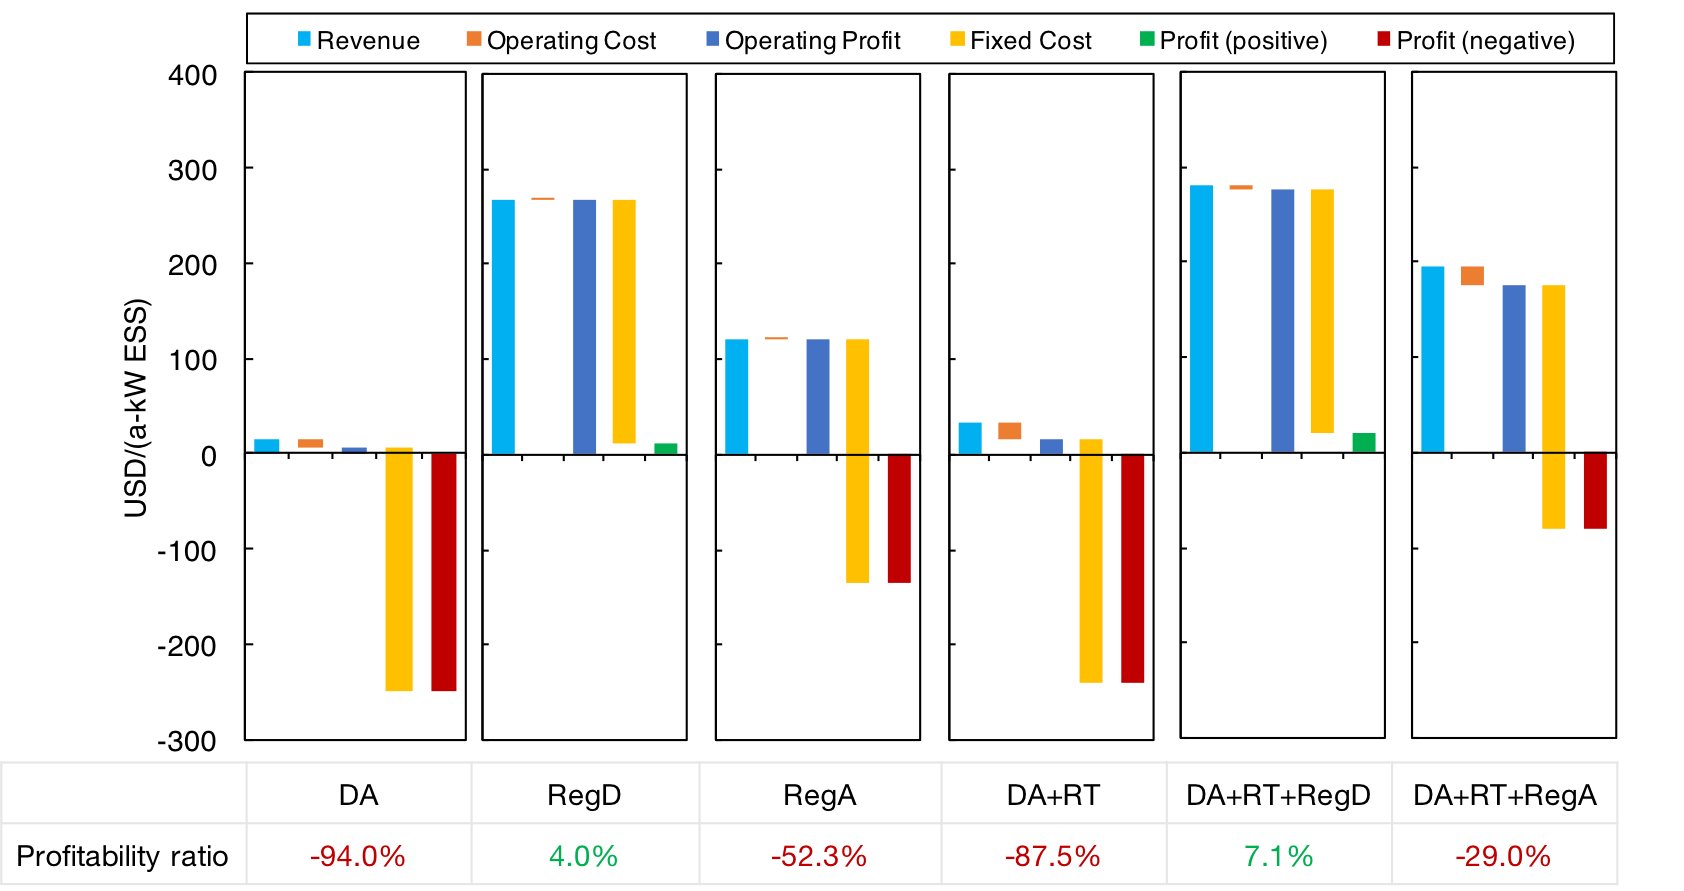
\includegraphics[width=0.9\linewidth]{Figures/PJM_ESS_profitability}
	\caption{Profitability of ESS in PJM electricity markets in the scenario of ``max. marginal Revenue"}
	\label{fig:pjm-ess-profitability}
\end{figure}

\begin{figure}[h!]
	\centering
	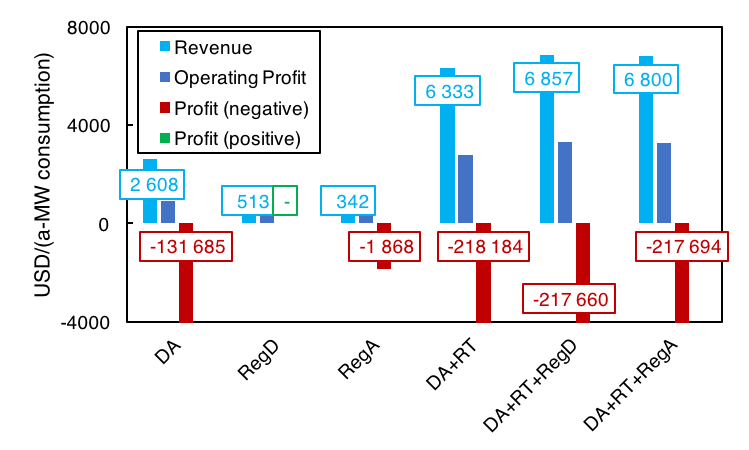
\includegraphics[width=0.9\linewidth]{Figures/PJM_ESS}
	\caption{Market size of ESS in PJM electricity markets in the scenario of ``max. Revenue"}
	\label{fig:pjm-ess}
\end{figure}

As we can clearly see, the RegD marketplace that is specially designed for emerging flexible technologies is indeed profitable. This shall give merit to PJM's RegD design including the conditional signal neutrality, operational flexibility, and higher price as a result of introducing mileage ratio and beneficial factor, as have sufficiently discussed in Section \ref{sec:qualitative-analysis}; also refer to Appendix \ref{sec:accounting-data-prepare}. The market with a total size of 513 USD/$(\text{a} \cdot \text{MW})$ can be wholly materialized by 2 kW/(MW consumption) BESSs without writing a loss, although the margin is very niche, barely above zero; see Figure \ref{fig:pjm-ess-profitable-size}.

\begin{figure}[h!]
	\centering
	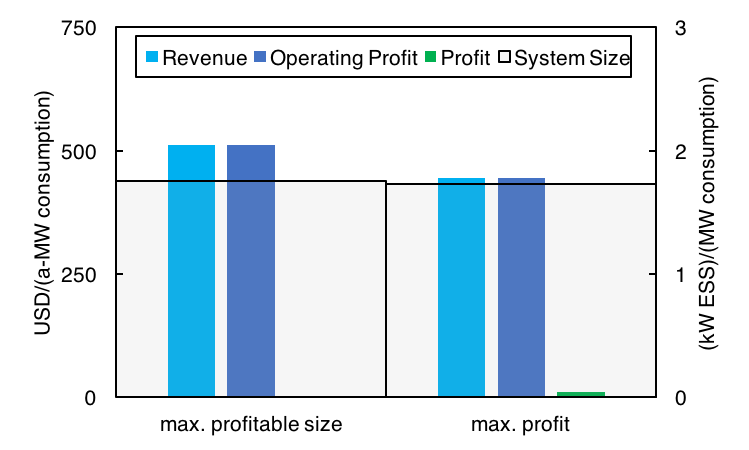
\includegraphics[width=0.9\linewidth]{Figures/PJM_ESS_profitable_size}
	\caption{Market size of ESS in PJM electricity markets in the scenario of ``max. System size with pos. Profit" and ``max. Profit"}
	\label{fig:pjm-ess-profitable-size}
\end{figure}

Those merits allow BESS players to offer RegD alone without coupled operations in the energy market which is currently necessary in Germany's power markets. As a result, stacking it with the energy market does not improve the profitability and tangible market size as significantly as in Germany. As we can see from an example shown by Figure \ref{fig:pjm-multitasking}, the system with pre-defined parameters in this study will have slightly surplus energy while strictly following the RegD signal. The SoC would raise quite slowly so that the resource can sustain the provision of RegD service over a long period (at least 84 hours shown in the chart) without involving transactions in energy markets. Trading in energy market is activated to leverage the arbitrage potential due to extreme price movements, which is however infrequent. Serving RegD is preferred for most of the time due its higher profitability. 

\begin{figure}[h!]
	\centering
	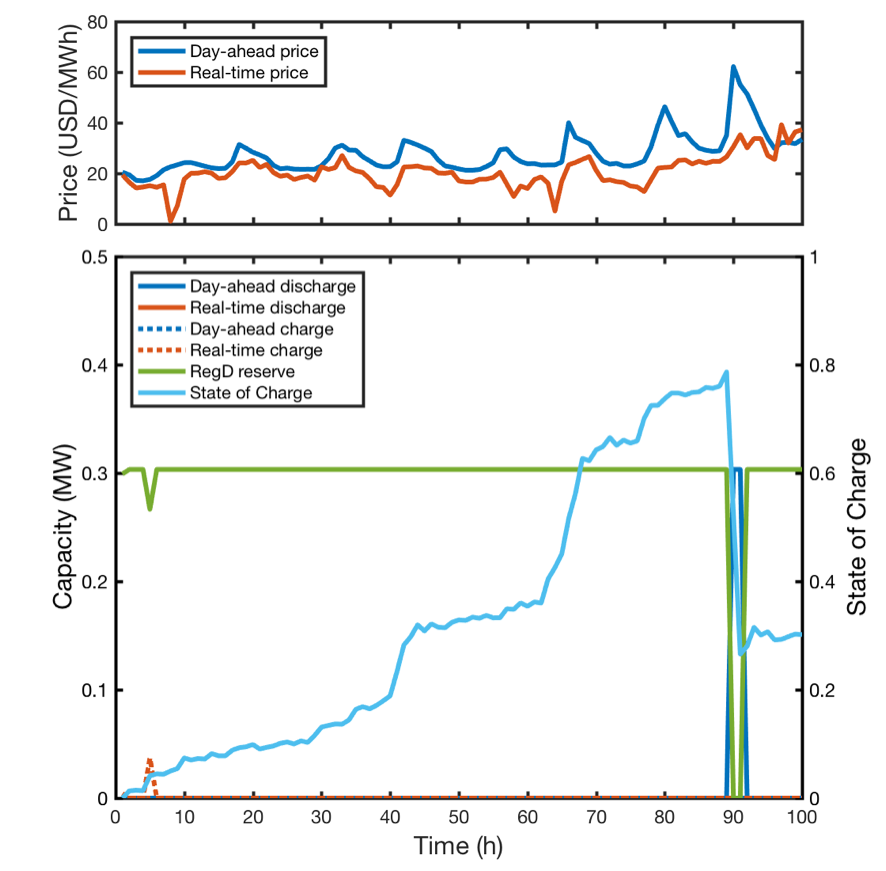
\includegraphics[width=0.9\linewidth]{Figures/PJM_multitasking_example}
	\caption{A example of operational plan with a 0.3MW battery energy storage system}
	\label{fig:pjm-multitasking}
\end{figure}

Apart from RegD market, there are no other profiting opportunities existing in PJM. Even the conventional regulation service RegA will create losses to BESS players.

Arbitrage in the energy market with flexibility through the so-called economic DR program, as is discussed in Section \ref{sec:qualitative-analysis}, is deemed not an ideal choice, especially in recent years when the electricity prices had fallen drastically with the shell gas revolution. As is discussed in Section \ref{sec:qualitative-analysis}, participating in the emergency DR program is a better option. However, the involvement of capacity market is not within our scope of quantifying the value, but the profiting mechanism is straightforward as is fully explained in the qualitative analysis. %It is also worthwhile to note that coupled operation in real-time and day-ahead markets will push the maximum revenue potential by 327 mUSD/a compared to 229 mUSD/a with participation in day-ahead market only.  

Overall, PJM shows a perfect example on how to offer incentives for the emerging storage technologies that are beneficial to the system, by implementing proper market frameworks such as the RegD and the  emergency DR program. For technology vendors, this market is already quite mature without spare space for new entrants unless significant changes may occur on market conditions, e.g. vast renewable penetration. Nonetheless, existing business cases in PJM may offer viable references for technology vendors to conduct similar practices in other markets. 

\subsubsection{ESS in NSW: most favorable market for arbitrage using flexibity yet still not profitable}

In New South Wales power markets, we only studied the real-time energy market, which was primarily due to the limitation of data availability.  Only information about total payment are available for the frequency control products. However, it was found that the overall size of these unaddressed markets are indeed negilible compared to the real-time energy market. The total payment for frequency control services in NSW was worth 23.4 mUSD (2933 USD/$(\text{a} \cdot \text{MW})$) in 2016, which was equal to just 0.53\% of the total payment in the real-time energy market that was 4.4 bUSD (\num{551516} USD/$(\text{a} \cdot \text{MW})$). It was also much smaller than merely the arbitrage value, being 2.7\% of the revenue from arbitrage of \num{109301} USD/$(\text{a} \cdot \text{MW})$ as shown by Figure \ref{fig:nsw-ess}. This reflects the philosophy of market design to fully exploit the ability of real-time energy market to response to the system imbalances which are otherwise tackled by frequency control markets\cite{AEMO2010}\cite{McConnell2015}.
As a result, the price volatility in NSW's real-time energy market is significantly higher than the energy markets in other geographies, as is shown by Table \ref{tab:price-3-geo}.

\begin{table}[h!]
	\centering
	\begin{tabular}{l l R{3cm} R{4.5cm}}
		\hline
		\textbf{Geography} & \textbf{Market} & \textbf{Average price (USD/MWh)} & \textbf{Standard deviation of price (USD/MWh)} \\
		\hline
		NSW  & RT & 46.0 & 86.0 \\
		\hline
		\multirow{2}{*}{Germany} & DA & 34.8 & 15.0 \\
		\multirow{2}{*}{} & RT & 35.1 & 16.1 \\
		\hline
		\multirow{2}{*}{PJM} & DA & 30.0 & 11.6 \\
		\multirow{2}{*}{} & RT & 27.6 & 14.8 \\
		\hline
	\end{tabular}
\caption{The average and standard deviation of energy price in three geographies}\label{tab:price-3-geo}
\end{table}

\begin{figure}[h!]
	\centering
	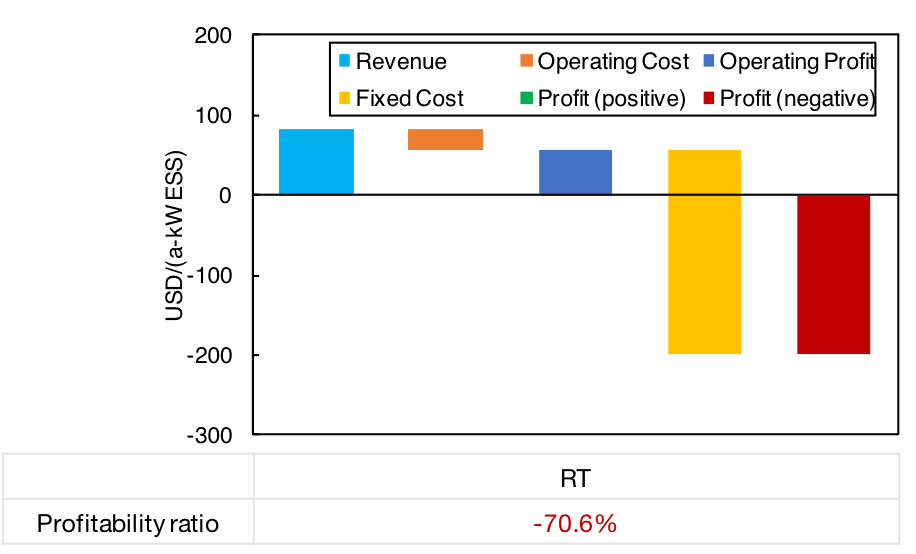
\includegraphics[width=0.9\linewidth]{Figures/NSW_ESS_profitability}
	\caption{Profitability of ESS in NSW electricity markets in the scenario of ``max. marginal Revenue"}
	\label{fig:nsw-ess-profitability}
\end{figure}

\begin{figure}[h!]
	\centering
	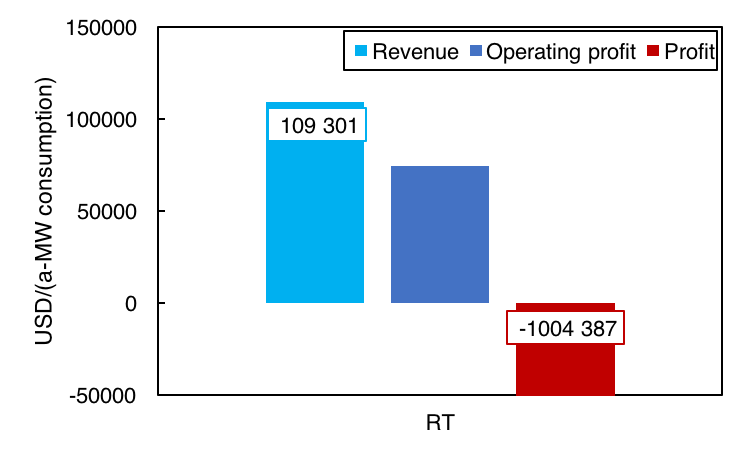
\includegraphics[width=0.9\linewidth]{Figures/NSW_ESS}
	\caption{Market size of ESS in NSW electricity markets in the scenario of ``max. Revenue"}
	\label{fig:nsw-ess}
\end{figure}

Such a volatile market is favorable for arbitrage. As we can see from Figure \ref{fig:nsw-ess-profitability} and \ref{fig:nsw-ess}.Profitability-wise the marginal revenue per unit system, 83 USD/$(\text{a} \cdot \text{kW ESS})$) is 2.4 times the value of arbitrage in DA+RT in PJM and 3.8 times the value of arbitrage in DA+ID in Germany. In terms of market potential, the maximum arbitrage revenue \num{109301} USD/$(\text{a} \cdot \text{MW})$) is roughly 17 times higher compared to either of those two arbitrage cases in Germany and PJM.

Nonetheless, even though in such a voltaile real-time energy market, it is still not a profitable business to deploy BESS in NSW for arbitrage.

\subsubsection{Cost reduction: where is the break-even point for arbitrage using BESSs}
According to the results above, using BESSs for balancing is already technically feasible while limitations lie on the aspect of market design. The value of arbitrage, however, is far away from being profitable due to high expenses on batteries. Overturn of arbitrage profitability using BESSs has to rely on reducing costs and changing market conditions. While the latter will be discussed in the proceeding section, hereby we present the results with reduced costs of battery stocks. 

In each geography, the case with the highest arbitrage potential was selected, which is respectively arbitrage in coupled day-ahead and intra-day market in Germany (DA+ID), arbitrage in coupled day-ahead and real-time market in PJM (DA+RT), arbitrage in real-time market in NSW (RT). The profitability is evaluated by the profitability ratio that is the ratio between the profit and overall costs including both operating and fix costs. We would show the maximum profitability ratio that is realized by a small size of BESS and meanwhile present the maximum profitable system size that is obtained as in the ``max. System Size with pos. Profit" described previously. 

\begin{figure}[h!]
	\centering
	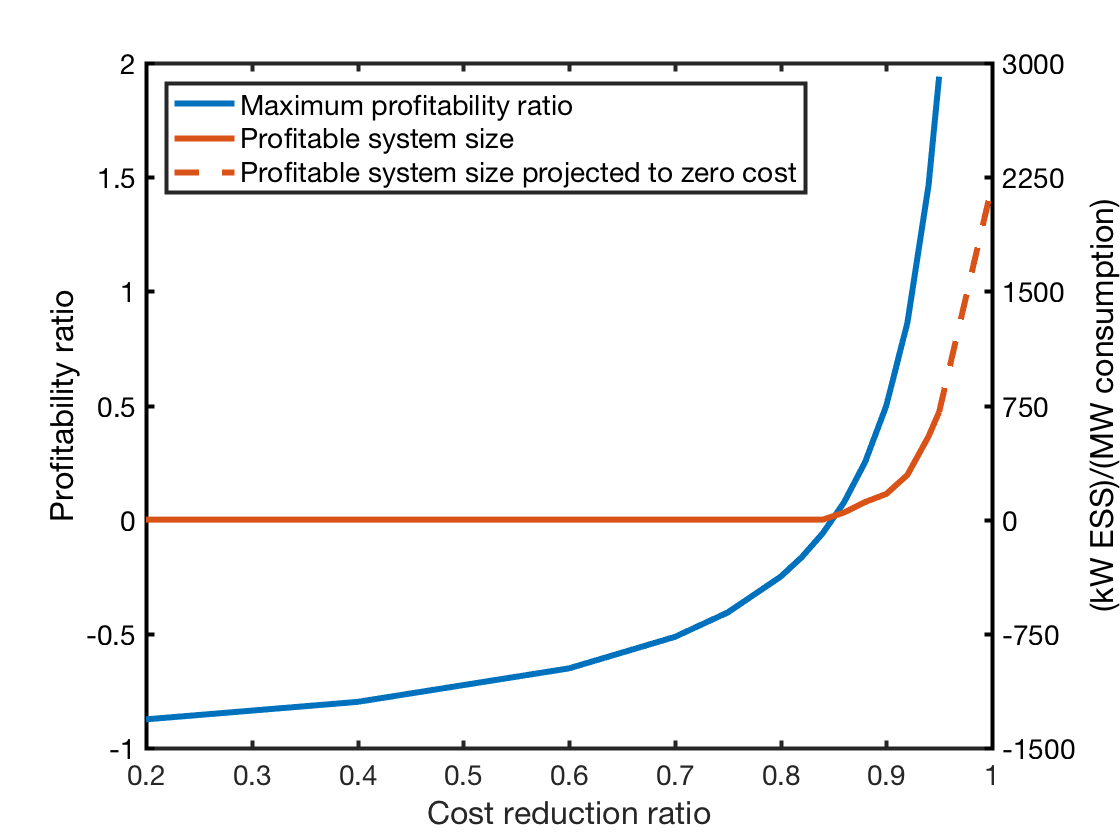
\includegraphics[width=0.9\linewidth]{Figures/CostReduction_Germany_ESS}
	\caption{Development of market size and profitability of arbitrage in coupled day-ahead and intra-day markets with reduced costs in Germany}
	\label{fig:germany-ess-costreduction}
\end{figure}

\begin{figure}[h!]
	\centering
	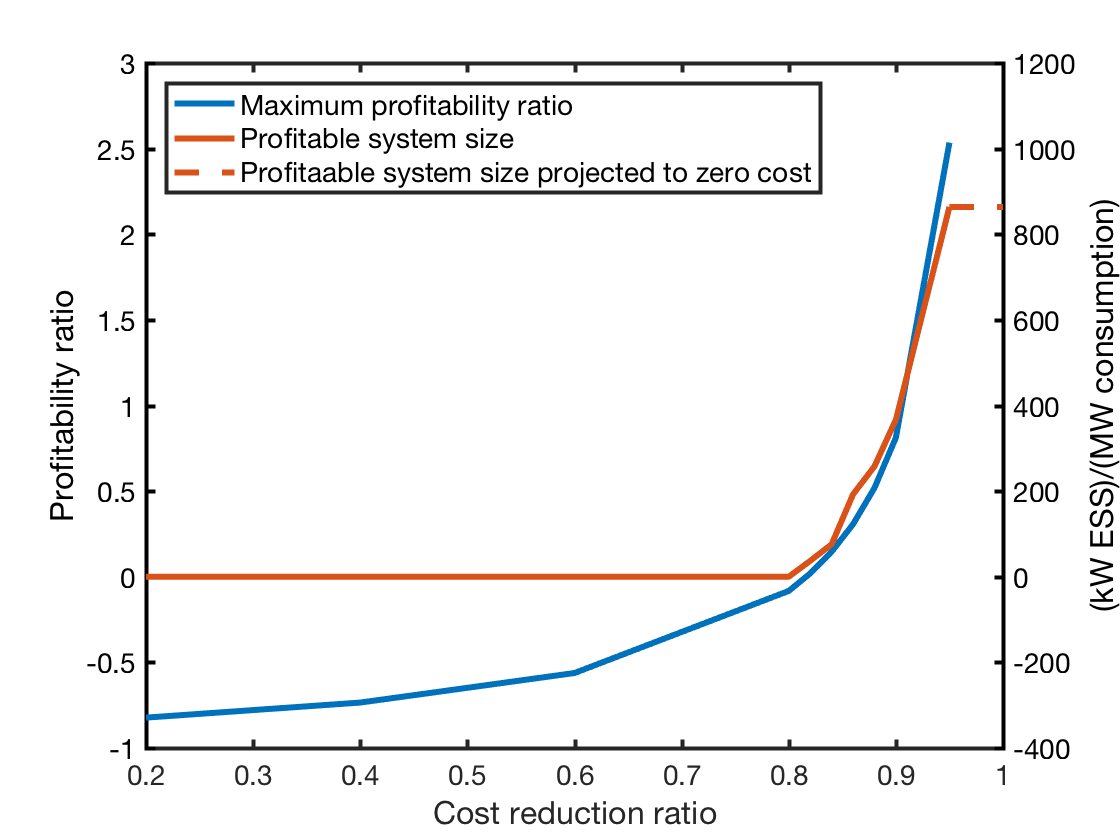
\includegraphics[width=0.9\linewidth]{Figures/CostReduction_PJM_ESS}
	\caption{Development of market size and profitability of arbitrage in coupled day-ahead and real-time markets with reduced costs in PJM}
	\label{fig:pjm-ess-costreduction}
\end{figure}

\begin{figure}[h!]
	\centering
	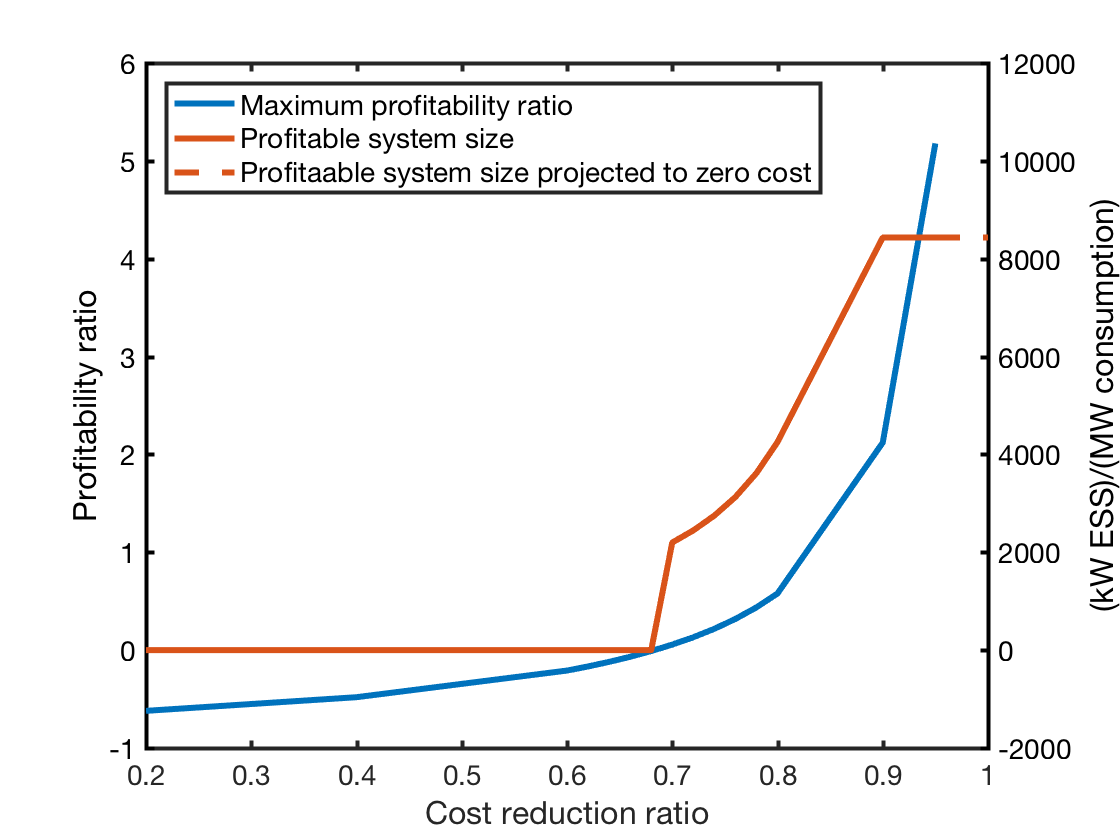
\includegraphics[width=0.9\linewidth]{Figures/CostReduction_NSW_ESS}
	\caption{Development of market size and profitability of arbitrage in real-time markets with reduced costs in NSW}
	\label{fig:nsw-ess-costreduction}
\end{figure}

Figure \ref{fig:germany-ess-costreduction} - \ref{fig:nsw-ess-costreduction} illustrate how the profitability and market size will evolve with cost reduced by up to 95\% in three geographies. The break-even point of costs is found to be 84\%, 81\% and 68\%, respectively in Germany, PJM and NSW. If we adopt the forecast made by IRENA\cite{IRENA2017} who predict the cost reduction by up to 60\% by 2030, none of these markets will be profitable for arbitrage by 2030. Even if we applied a constant learning rate of 14\% per annum according to \cite{Nykvist2015}, the break-even point will be realized in 12, 11 and 8 years, respectively in Germany, PJM and NSW. 

Moreover, it shall be noticed while the break-even point is just reached, the total profitable system size will be almost at zero. To materialize the whole potential of arbitrage revenue, it requires a cost reduction of 95\%+, 95\% and 90\%, respectively in Germany, PJM and NSW, which is almost impossible to be realized in the foreseeable future.

As a conclusion, the cost reduction of BESS by learning effect alone will not turn over the profitability of arbitrage using BESSs in the near future. Unless revolutionary technical innovations happen, opportunities of arbitrage using BESS may only arise with drivers from the market, e.g. renewable penetrations, which are to be shown in Section \ref{sec:impact-market-condition}.

\subsubsection{EV2G  in Germany: promissing and fast-growing opportunities}
Implementing EV as a grid resource is not as straightforward as using generic ESSs that is discussed above. The main issue is that the energy demand for EV driving itself poses challenges to grid. It is not possible to deliver any services without incorporate a large-volume energy market. Therefore, the day-ahead energy market is always included for all the cases for EV2G. Moreover, in our case studies, it is found even with the day-ahead market, charging the EVs is not feasible while their number reached a certain level. In the optimization framework, the technology constraints would violate market constraints, especially the one that we set to restrict the activation of peak generation during non-peak hours, while the EV fleet grows beyond a certain scale. This corresponds to the situation where spare generation resources in the power system are not sufficient  to fulfill the energy needs of EVs. The electricity price may raise significantly in those scenarios compared to nowadays's level. As is shown by Figure \ref{fig:EV_nan_percentageg}, when the number of EV is higher than 1 million, it start to stress the electricity supply if the generation capacity remains at present level. 
\begin{figure}[h!]
	\centering
	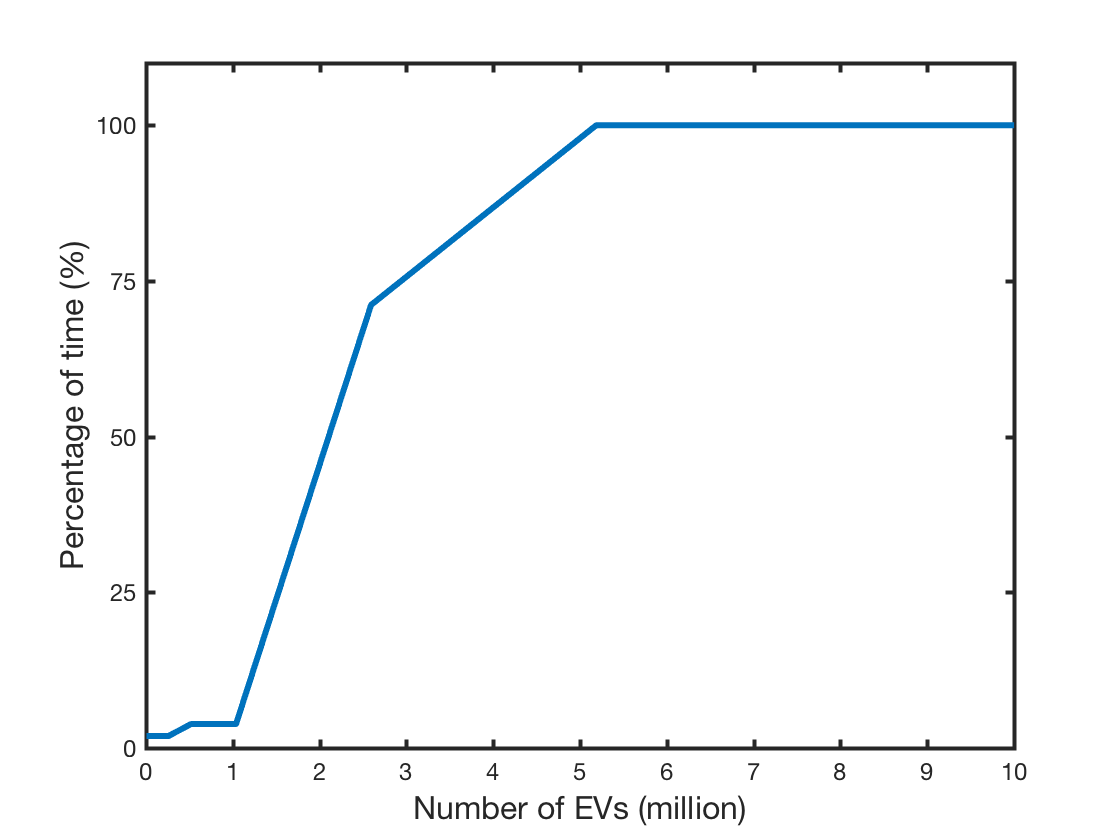
\includegraphics[width=0.95\linewidth]{Figures/EV_nan_percentage}
	\caption{Percentage of time when EV charging demand cannot be fulfilled in Germany}
	\label{fig:EV_nan_percentageg}
\end{figure}

This finding implies when there will be 1 million more EVs in Germany compared to the number in 2016, it will create great incentives for infrastructure extension of electricity grid, which reveals a promising business opportunity. Nevertheless, studies under that condition is beyond the focus of our work. Instead, we would only perform scenario analysis when the number of EV is within the limit of 1 million. 

In this thesis, we applied three scenarios studying the EV2G market in Germany:

\begin{itemize}
	\item \textbf{EV number 2016:} assuming all  EVs in Germany by 2016 are contract for delivering EV2G services
	\item \textbf{EV number 2017:} similar to the first scenario but using the data of 2017
	\item \textbf{2\% market share:} assuming EVs will account for 2\% of the total vehicle number in Germany (45 million according to \cite{Eurostat_de_v}) i.e. 0.9 million EVs in the future
\end{itemize}

According to the Federal Motor Transport Authority of Germany (Kraftfahrt-Bundesamtes, KBA)\cite{KBA2017}, the number of plug-in electric vehicles has grown fast over the past year, especially in 2017. Since the EV registered before 2010 is negligible, we conceived the cumulative registration since 2010 as the total number of EVs in Germany, shown as Figure \ref{fig:Germany_EV_number}.

\begin{figure}[h!]
	\centering
	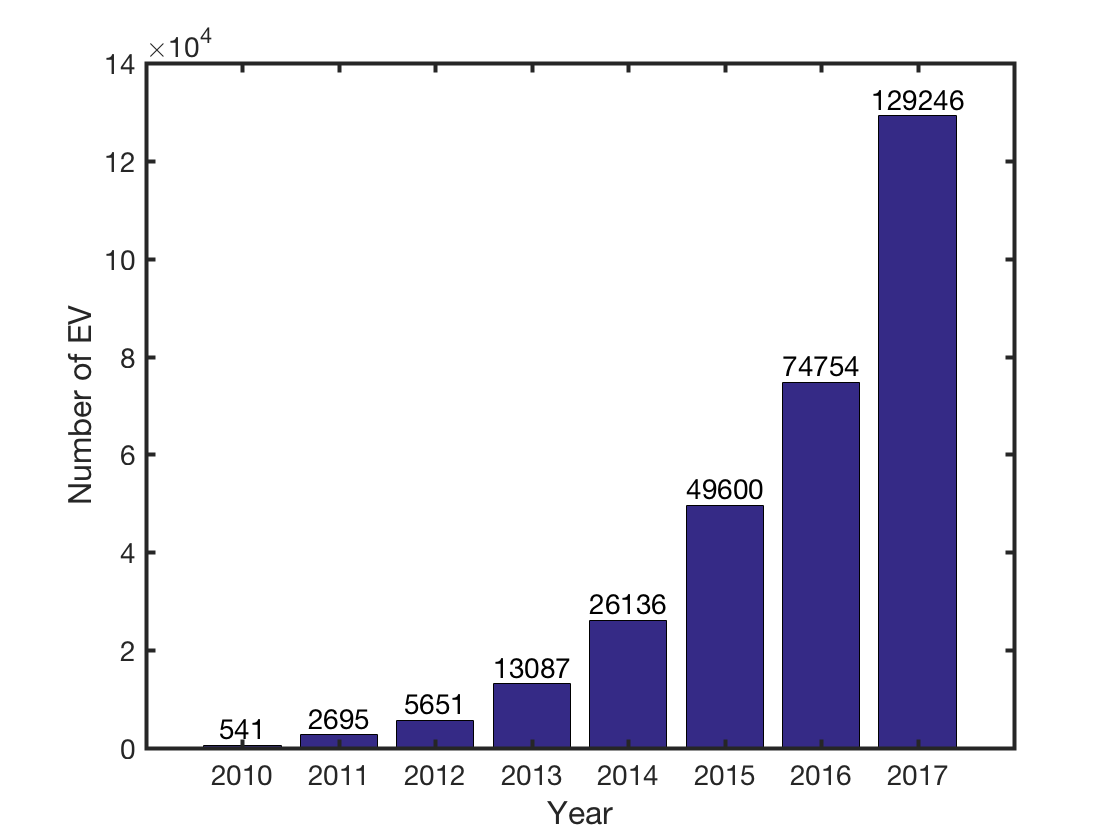
\includegraphics[width=0.95\linewidth]{Figures/Germany_EV_number}
	\caption{Cumulative registration of plug-in electric vehicles in Germany since 2010 \cite{KBA2017}}
	\label{fig:Germany_EV_number}
\end{figure}

The numbers of EV that were taken for the scenario analysis are then determined and list in Table \ref{tab:ev-number-scenario-germany}.

\begin{table}[h!]
	\centering
	\begin{tabular}{l r r}
		\hline
		\textbf{Scenario} & \textbf{EV number total} & \textbf{EV number per household} \\
		%\hline
		\hline
		EV number 2016 &  \num{74754} & \num{0.014} \\
		EV number 2017 &  \num{129246} & \num{0.025} \\
		2\% market share &  \num{900000} & \num{0.174} \\
		\hline
	\end{tabular}
\caption{The number of EV for each scenario in Germany}\label{tab:ev-number-scenario-germany}
\end{table}

\begin{figure}[h!]
	\centering
	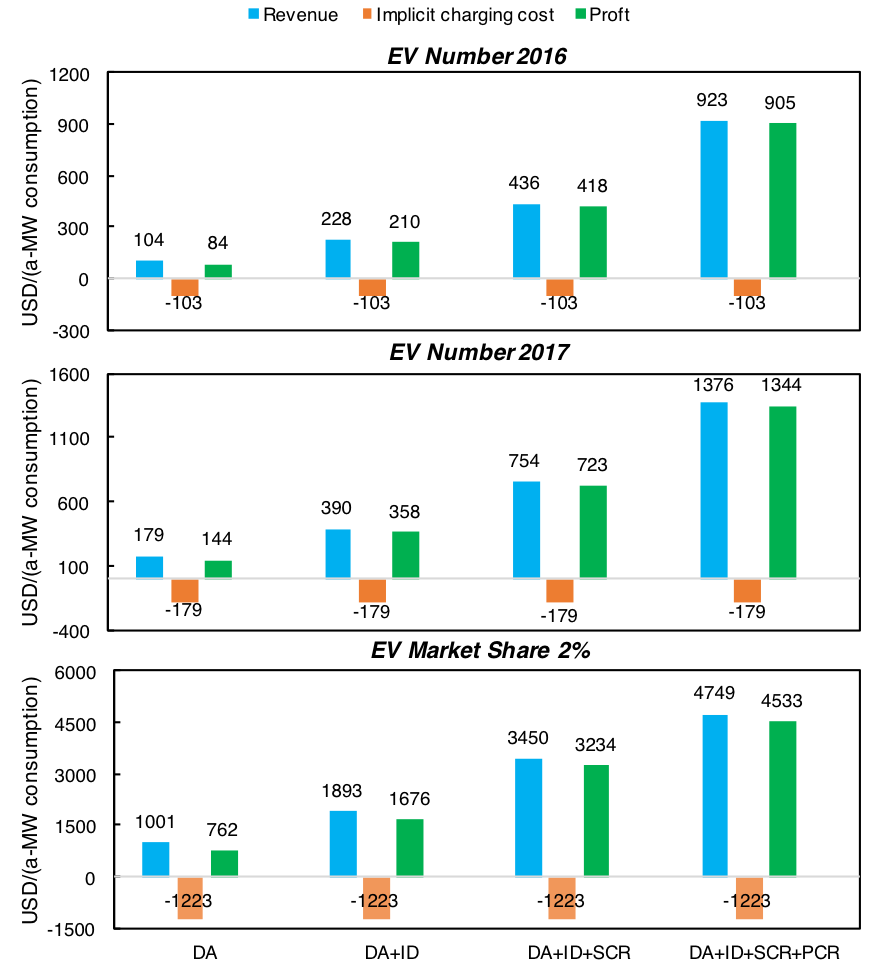
\includegraphics[width=0.95\linewidth]{Figures/Germany_EV_profit}
	\caption{Market size and profitability of EV2G in Germany electricity markets}
	\label{fig:Germany_EV}
\end{figure}

Based on these scenarios, we performed the case studies and the results are shown by Figure \ref{fig:Germany_EV}. All the business cases reported profits, especially the cases where frequency control markets were coupled. Furthermore, as we seen from the charts, the drastic growth of EVs was reflected on the growth of EV2G market potential from 2016 to 2017, and there are still much more growth space till the scenario of 2\% EV market share. However, it shall be noticed that our analysis has overlooked some factors which could make the business less profitable as shown here. The main issue is that we use a determinate approach to simulate the frequency control signal and EV driving behaviors which eliminated the risks of failing to deliver the frequency control services as planned. Alipour \textit{et. al.}\cite{Alipour2017} made a study on EV2G for frequency control services with a stochastic approach. It was found in a case where a profit of 7980 USD was expected, the conditional value-at-risk was 5720 USD, indicating the risking nature of such a business. In the outlook of this thesis, we proposed a stochastic method by using Markov chain to simulate the uncertain driving behavior of EVs and then the estimation of risk can be conducted. Nonetheless, while quantitative risk assessment against uncertainty is necessary for designing a specific project, it is beyond the focus of a study understanding the whole market value so is not included in our study. Besides, the battery degradation incured by EV driving was not included here while in reality it would be a challenging issue to account the degradation caused by providing EV2G services separately from driving. Finally, implementing EV2G for frequency control is not a mature technology due to its complexity\cite{Peng2017}\cite{Shafie-Khah2015}\cite{Bessa2014}\cite{Bessa2013}, which implies a high research and development cost.

It is also worthwhile to note that while the number of EVs (0.9 million ) in the scenario of ``2\% Market Share" has reached the edge of the affordable level (1 million) for the grid, revenues are significantly smaller than the maximum potential revenues derived in the case studies of ESSs. The shares of maximum achievable revenue by EV2G to the total market potential by generic ESS were between 25\%-50\% among different cases. This reveals that constrained by the limitations discussed above, EV2G will not be able fully cover the needs for flexibility by its own, even on a aggregated system level without considering the distributed manners. Other types of flexibility would still be necessary to complement the demands for flexibility in scenarios with high EV penetrations.

\subsubsection{EV2G  in PJM: RegD market would be saturated shortly if EV2G was indeed implemented}

\begin{figure}[h!]
	\centering
	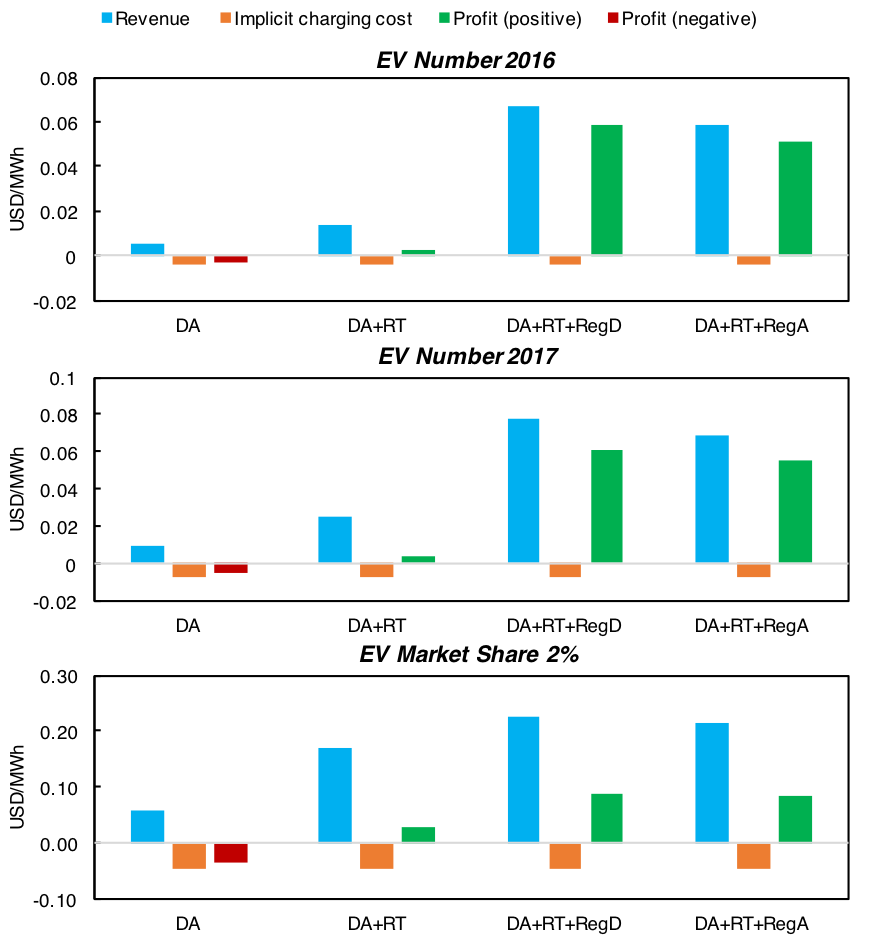
\includegraphics[width=0.95\linewidth]{Figures/PJM_EV_profit}
	\caption{Market size and profitability of EV2G in PJM Electricity markets}
	\label{fig:PJM_EV}
\end{figure}

Similar studies are performed in PJM power markets. Since the geographic coverage of PJM is not strictly corresponding to the administrative divisions, it becomes a extremely sophisticated task to get the official number of EVs in PJM with the public data. Therefore, we projected the number in Germany to PJM by their ratio of household number. That means, in the corresponding scenarios, the EV ownership per household is identical in Germany and PJM. We took this approach to make an indication of the market value, which however shall be noticed with caution that it may deviate from real conditions. 
Table \ref{tab:ev-number-scenario-PJM} shows the number of EV in each scenario.

\begin{table}
	\centering
	\begin{tabular}{ l r r }
		\hline
		\textbf{Scenario} & \textbf{EV number total} & \textbf{EV number per household} \\
		%\hline
		\hline
		EV number 2016 &  \num{43713} & \num{0.014} \\
		EV number 2017 &  \num{75578} & \num{0.025} \\
		2\% market share &  \num{526290} & \num{0.174} \\
		\hline
	\end{tabular}
	\caption{The number of EV for each scenario in PJM}\label{tab:ev-number-scenario-PJM}
\end{table}

With these numbers of EV, no generation shortage was observed, expect for only one week in the scenario of 2\% EV market share. The results in that week were discarded, i.e. no operations and thus no revenues in that week. This accounts for approximately 2\% of the time in a year so the impact on final results shall be negligible.

Figure \ref{fig:PJM_EV} summarizes the results of cases in PJM. The revenue potential in energy-only cases are much smaller compared to the corresponding results in Germany, which is mainly because the values were dilluted by higher consumption rate per household (MP) in PJM (2.5 times the value in Germany referring to Table \ref{tab:MP}). 

However, the incremental revenue by stacking RegD to DA+RT case was 455 USD/$(\text{a} \cdot \text{MW})$ in the scenario of ``EV Number 2016" while the addtional revenue by stacking SCR to DA+ID in Germany was merely 208 USD/$(\text{a} \cdot \text{MW})$, which again reveals the favor of RegD toward flexibility resources. 

Noticing that the whole RegD market potential for generic flexiblity resources is merely 513 USD/$(\text{a} \cdot \text{MW})$ as was shown previously by \ref{fig:pjm-ess}.This market could be easily exhausted by a small size of EV fleet. 
 
\subsubsection{EV2G  in NSW: a small portion of arbitrage potential to be capturned by EV2G yet still much valuable than in other geographies}

Using the same methodology as in PJM, scenarios are established by taking the identical EV numbers per household, as is shown by Table \ref{tab:ev-number-scenario-nsw}.

\begin{table}[h!]
	\centering
	\begin{tabular}{ l r r }
		\hline
		\textbf{Scenario} & \textbf{EV number total} & \textbf{EV number per household} \\
		%\hline
		\hline
		EV number 2016 &  \num{4849} & \num{0.014} \\
		EV number 2017 &  \num{8383} & \num{0.025} \\
		2\% market share &  \num{58377} & \num{0.174} \\
		\hline
	\end{tabular}
	\caption{The number of EV for each scenario in NSW}\label{tab:ev-number-scenario-nsw}
\end{table}

\begin{figure}[h!]
	\centering
	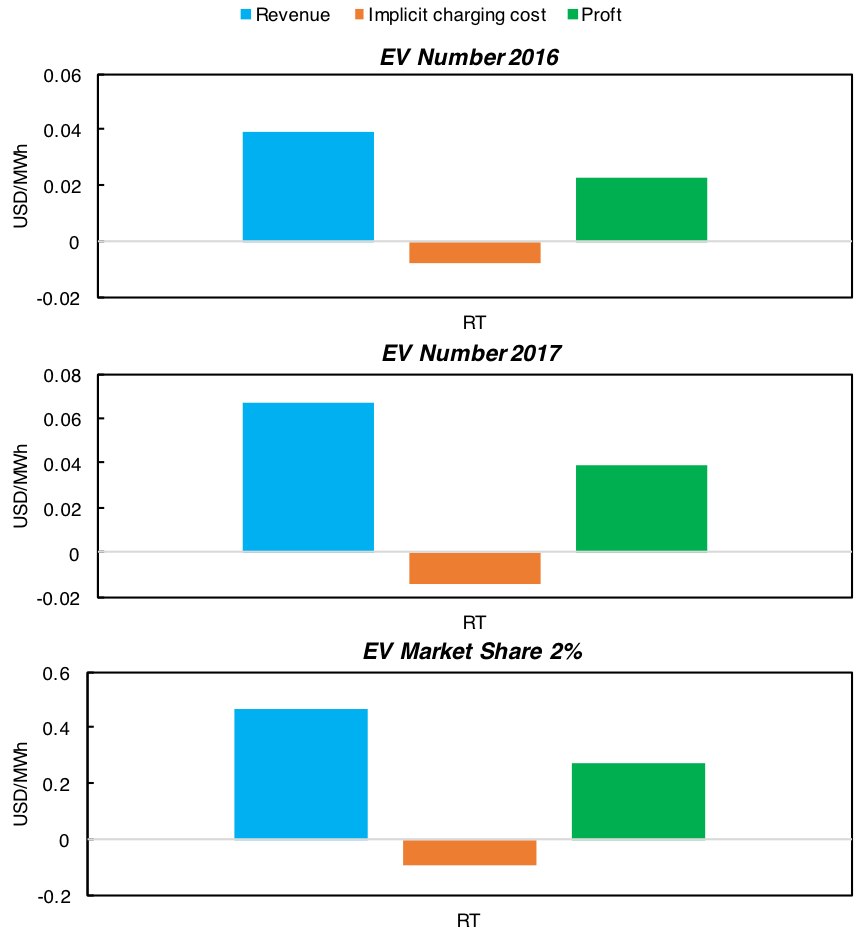
\includegraphics[width=0.95\linewidth]{Figures/NSW_EV_profit}
	\caption{Market size and profitability of EV2G in NSW Electricity markets}
	\label{fig:NSW_EV}
\end{figure}

Figure \ref{fig:NSW_EV} presents the results of three scenarios in NSW's real-time energy market. Although the size of EV fleet is merely 6.5\% of that in Germany and 11.1\% of that in PJM. The market sizes are generally on the same scale as the other two markets. The revenue per EV of around 560 USD/a and profit per EV of about 365 USD/a are significantly higher than other geographies, as a result of the price volatility in NSW's real-time market discussed previously. High unit return provides more incentives of the end-users to participate in the EV2G program, which makes the business more realizable.

Besides, it can be noticed the overall market size even in the last scenario where we see a revenue potential of 32.8 USD/a accounts for a small portion of the total arbitrage potential in NSW's real-time market revealed in the section for generic ESSs, leaving a vast space for other technologies.3.8\%

\subsubsection{Conclusion}



\subsection{Impact analysis of changing market conditions}
\label{sec:impact-market-condition}


\subsubsection{Model setup and validation}
As is introduced in Section \ref{sec:market-simulation}, the market simulation module was designed to generate price scenarios with changed market conditions so that we can analyze the future trend of market value by understanding potential impacts of certain key factors. 

The module is developed using the methodology in Section \ref{sec:market-simulation} and based on day-ahead market and generation data in Germany in 2016.

First of all, the data of Germany day-ahead price and volume were collected and shown as Figure \ref{fig:merit-orignal}.

\begin{figure}[h!]
	\centering
	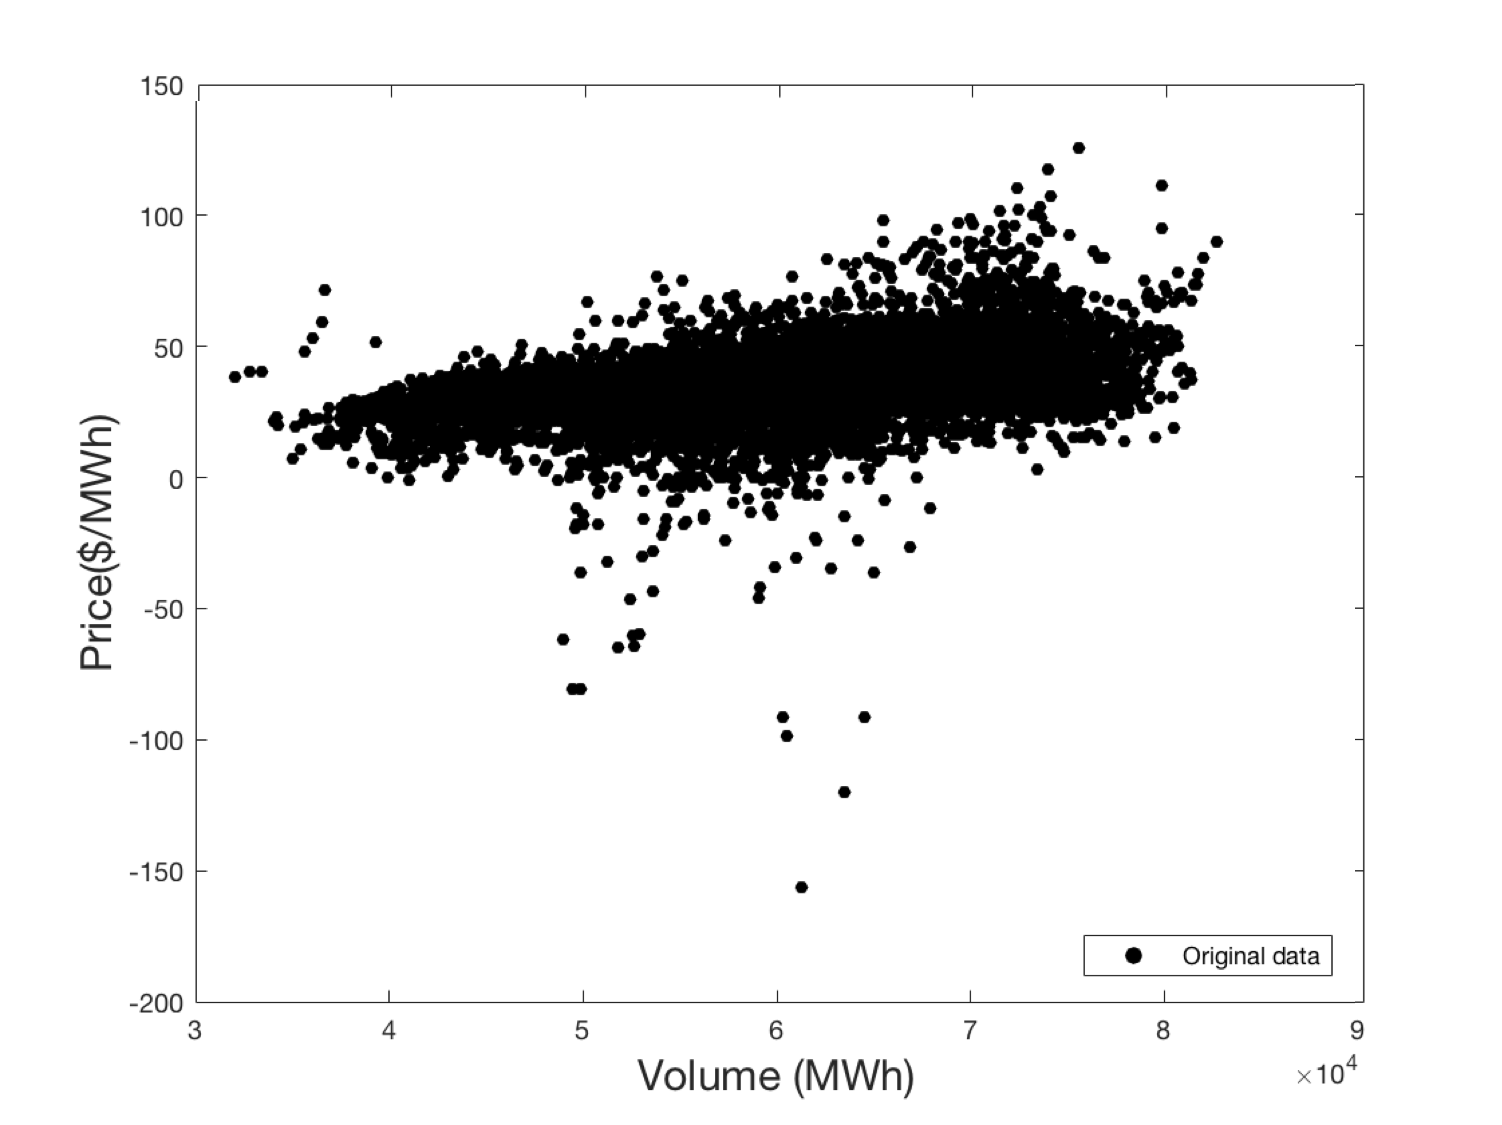
\includegraphics[width=0.95\linewidth]{Figures/Merit-order-original}
	\caption{Germany day-ahead price-volume data in 2016}
	\label{fig:merit-orignal}
\end{figure}

The pattern of merit-order effect is not clearly recognizable from the original data mainly due to the disturbs of variable renewable generation which has raised significantly in past years. This prevents us from directly applying merit-order models developed by previous studies\cite{He2013}\cite{Grunewald2012a}. Therefore, we applied the algorithm described in Section \ref{sec:market-simulation} which take into account the renewable generation and bounded flexibility of conventional generations. Figure \ref{fig:merit-transformed} shows the transformed pattern of data where a clearer merit-effect is identifiable. Figure \ref{fig:merit-classified} projects the classification to the original data distribution and it can be seen that the algorithm has successfully separated the data points where the price was driven to be higher or lower than average level due to the uplift effects introduced in \ref{sec:market-simulation}. 

\begin{figure}[h!]
	\centering
	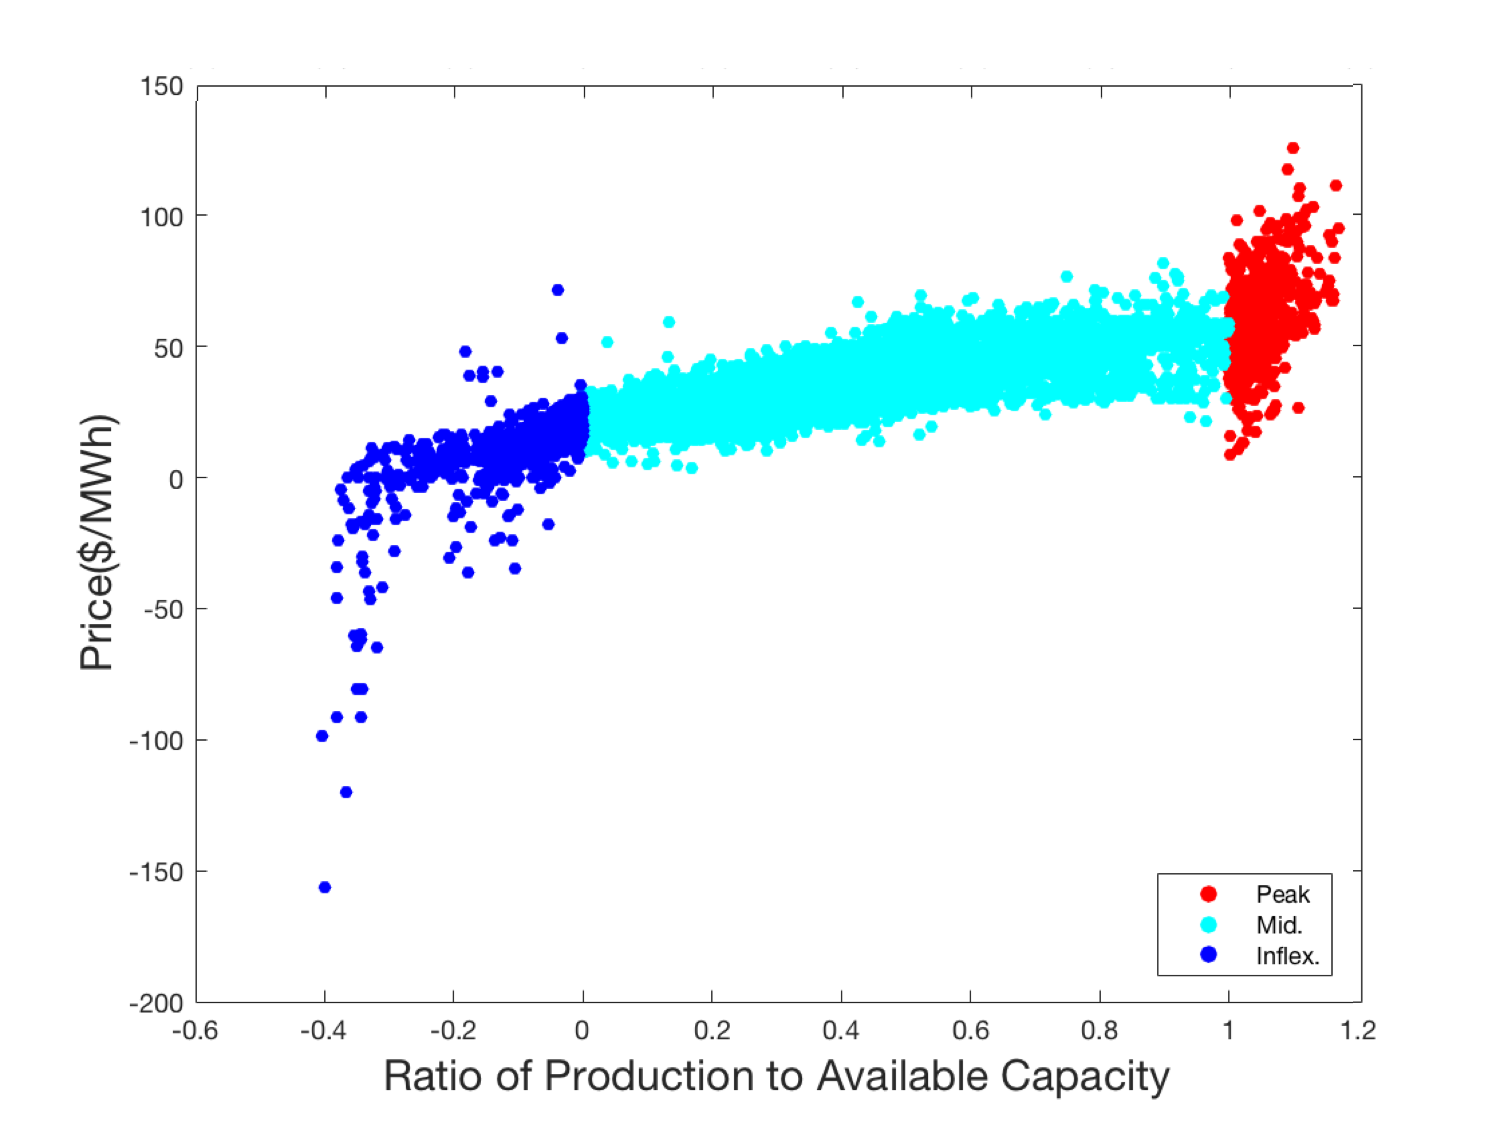
\includegraphics[width=0.95\linewidth]{Figures/Merit-order-transformed}
	\caption{Transformed pattern of Germany day-ahead price-volume data in 2016}
	\label{fig:merit-transformed}
\end{figure}
\begin{figure}[h!]
	\centering
	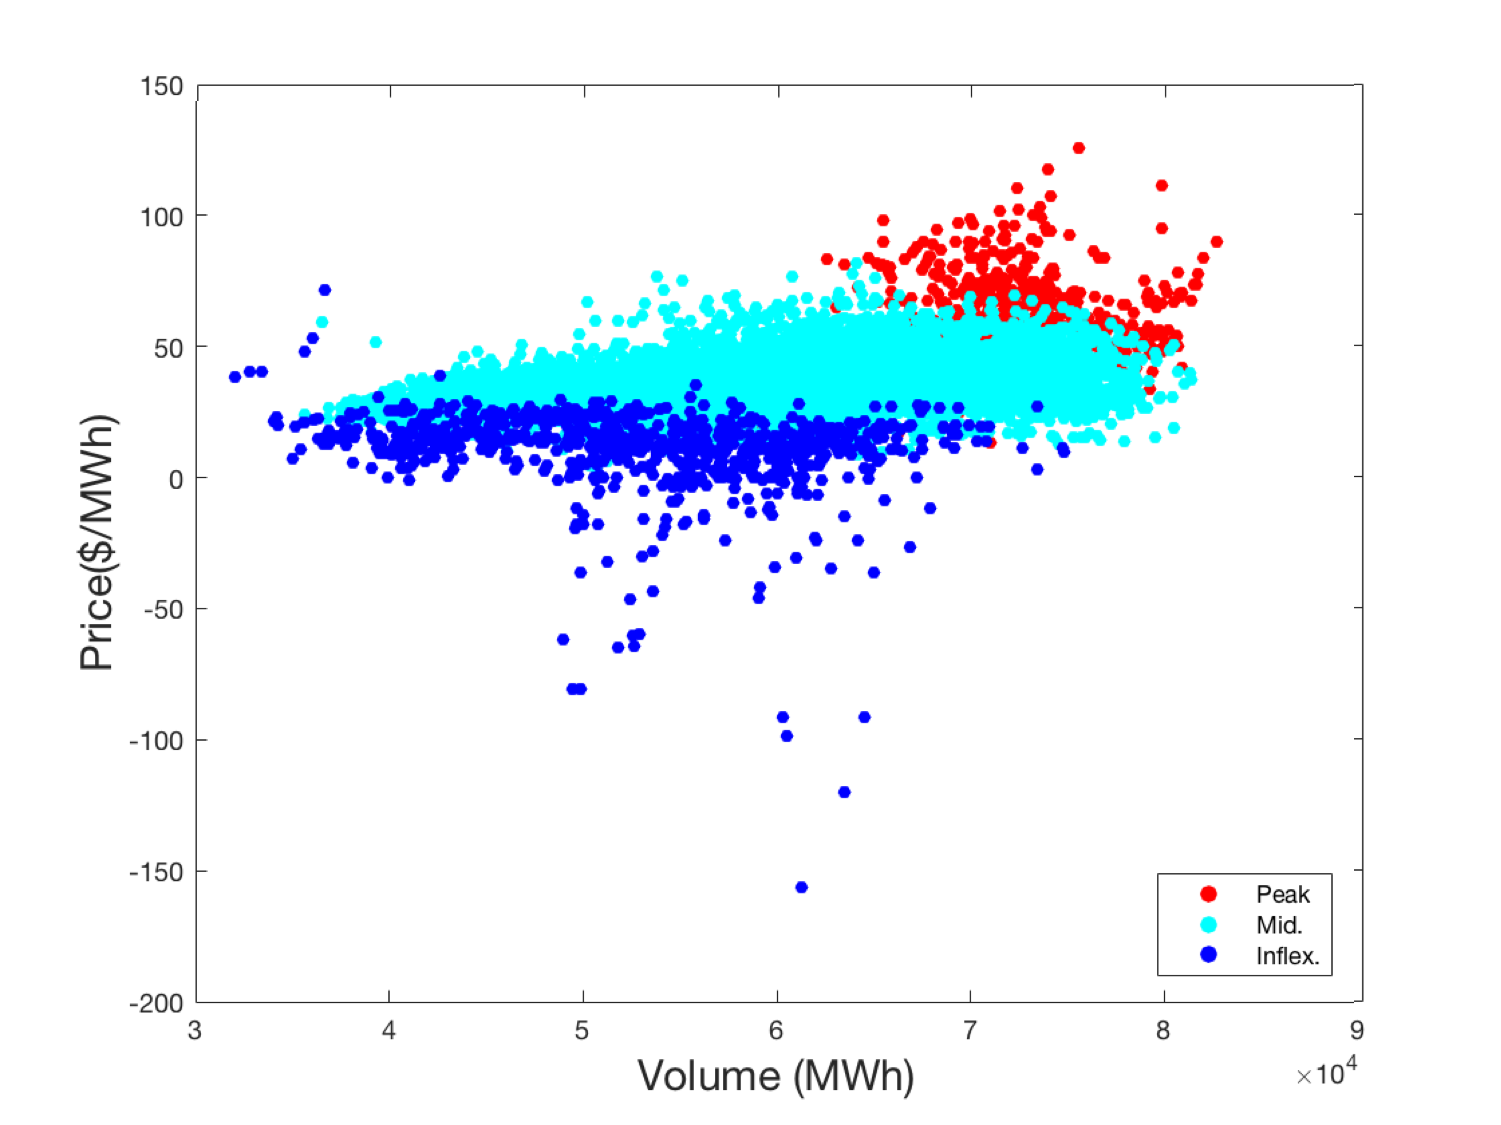
\includegraphics[width=0.95\linewidth]{Figures/Merit-order-classified}
	\caption{Classification of Germany day-ahead price-volume data in 2016}
	\label{fig:merit-classified}
\end{figure}

Thereafter, we fitted the transformed data pattern with the piece-wise function defined by \eqref{eq:merit-order-model}. The estimated parameters are listed in Table \ref{tab:merit}. The fitted merit-order curve is illustrated by Figure \ref{fig:merit-fitted} and distribution of errors between the fitted price and actual price is shown by Figure \ref{fig:merit-error}.

\begin{table}[h!]
	\centering
	\begin{tabular}{|l | r r r|}
		\hline
		Class & \multicolumn{3}{c|}{Parameters}\\
		\hline
		 & $a$ & $b$ & $c$\\
		\hline
		\hline
		Inflex. & 17.05 & -1.49 & -12.35 \\
		\hline
		\multirow{3}{*}{Mid.} & 48.66 & 16.40 & \\
		\multirow{3}{*}{} & 38.04 & 20.12 & \\
		\multirow{3}{*}{} & 16.37 & 34.20 & \\
		\hline
		Peak & -194.95 & 491.46 & -0.69 \\
		\hline
	\end{tabular}
	\caption{Parameters of the merit-order model}\label{tab:merit}
\end{table}

\begin{figure}[h!]
	\centering
	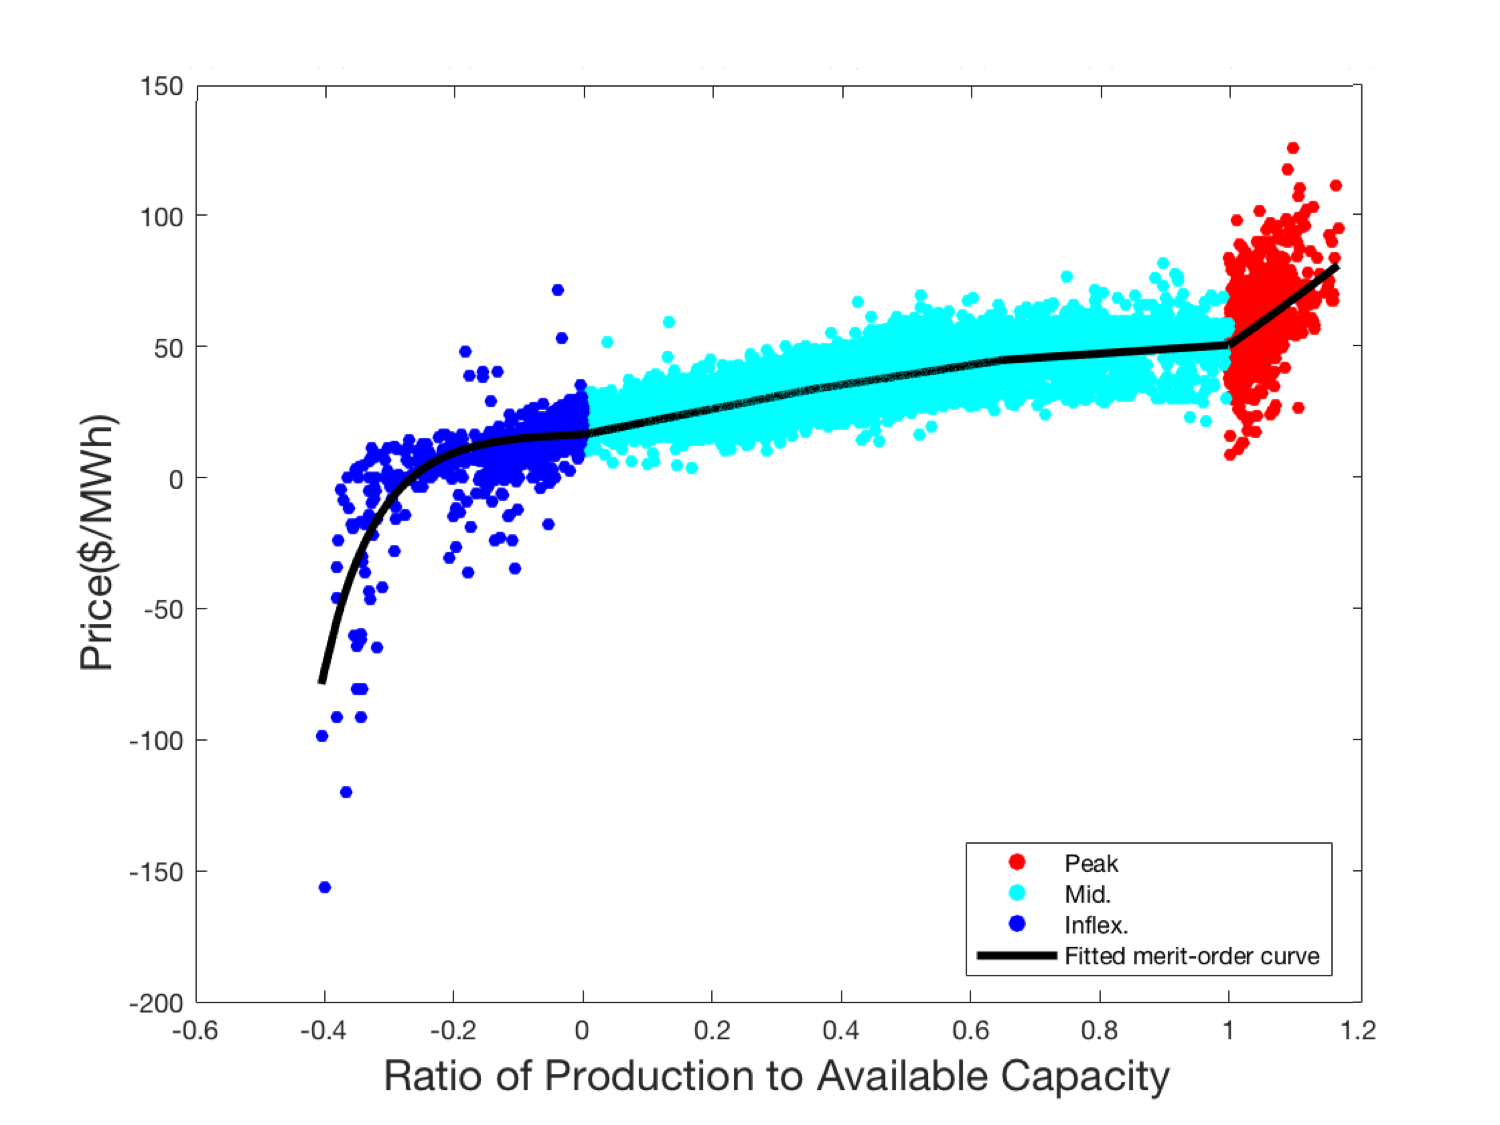
\includegraphics[width=0.95\linewidth]{Figures/Merit-order-fitted}
	\caption{Fitted merit-order curve with Germany day-ahead price-volume data in 2016}
	\label{fig:merit-fitted}
\end{figure}

\begin{figure}[h!]
	\centering
	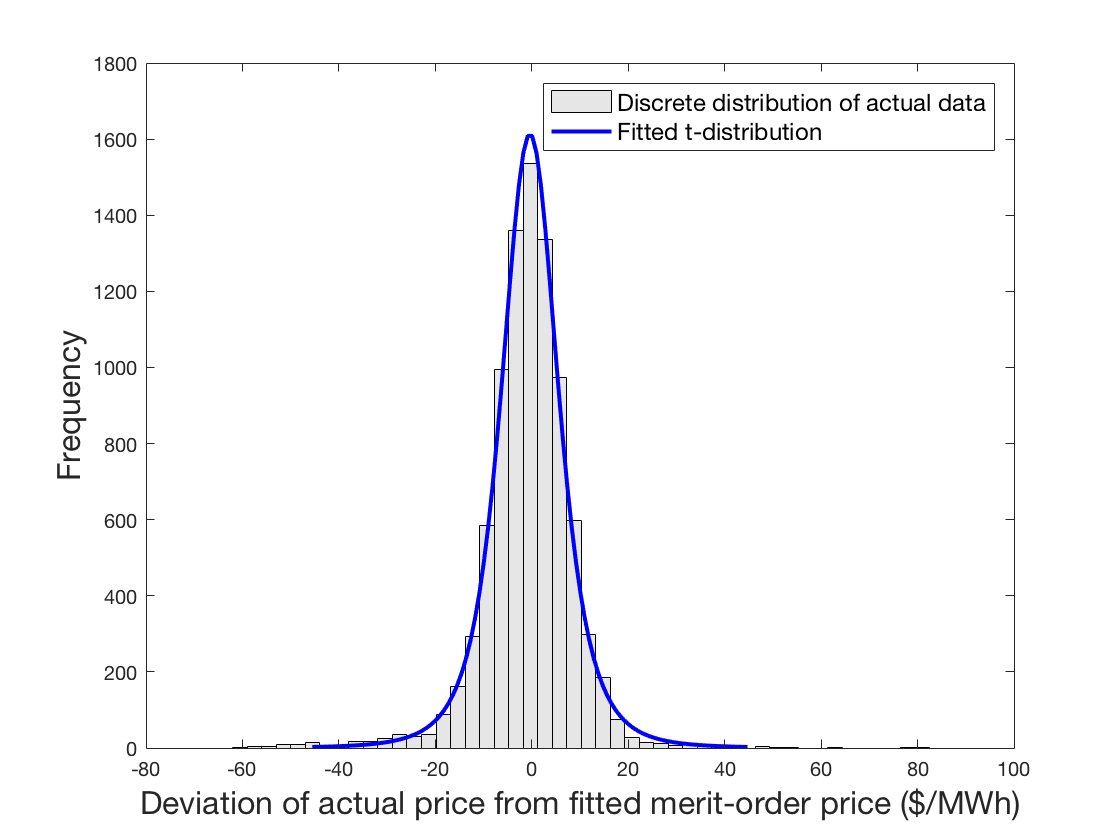
\includegraphics[width=0.95\linewidth]{Figures/4_Error-distribution}
	\caption{Distribution of errors between fitted merit-order price and actual price}
	\label{fig:merit-error}
\end{figure}

We simulated the day-ahead price using this merit-order model and compared to the actual market data. It can seen from Figure \ref{fig:merit-fitted}-\ref{fig:merit-error} that while the fitted merit-order price shows a good fitness to the actual price in terms of general trend, the stochastic movements of the price are eliminated. Merely with the merit-order model, a smoothed curve of price time-series would be generated where the drastic jumps of price cannot be captured, as is demonstrated by Figure \ref{fig:price-example}.

\begin{figure}[h!]
	\centering
	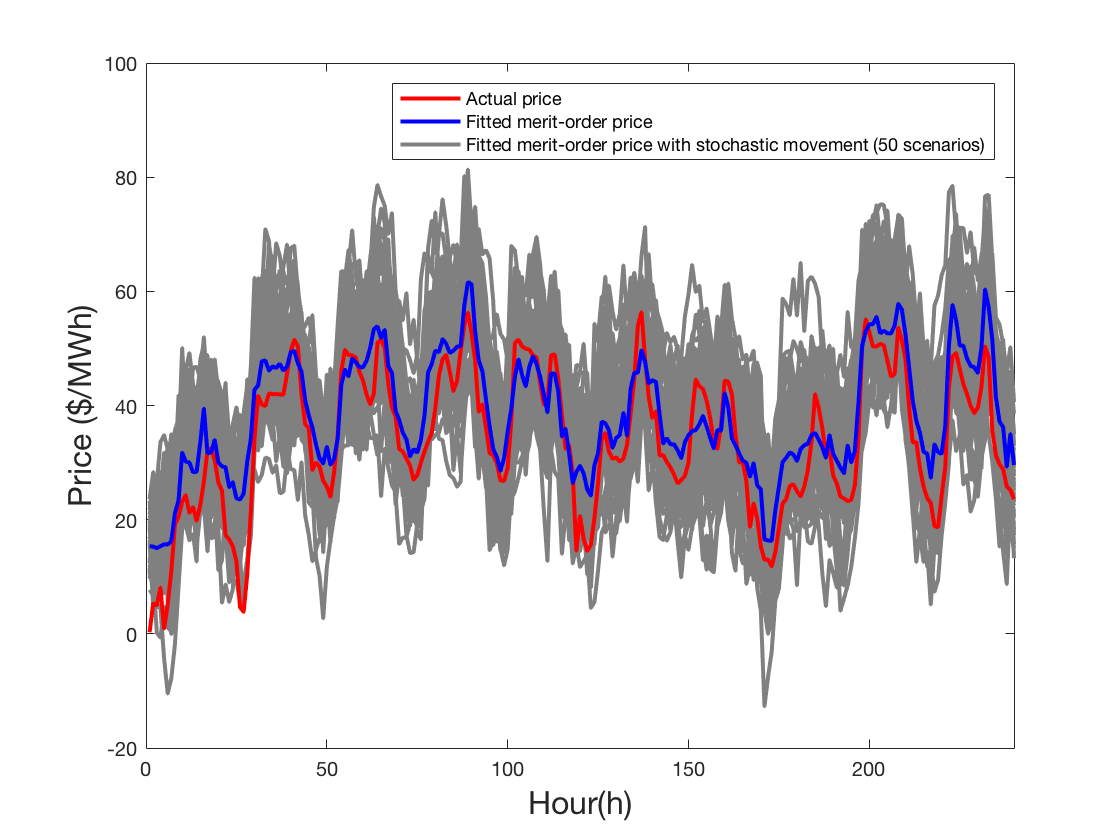
\includegraphics[width=0.95\linewidth]{Figures/5_Example-simulated_price}
	\caption{Generated price scenarios}
	\label{fig:price-example}
\end{figure}

Unlike studies on valuation of a conventional generation resources where such a merit-order model may suffice, the elimination of stochastic price movement would reduce the value of arbitrage greatly as is shown by Figure \ref{fig:model-validation}. This shall be understood intuitively as arbitrage activities pick the price differences among different trading slots and less volatile price movements would certainly affect the value creation of arbitrage.

\begin{figure}[h!]
	\centering
	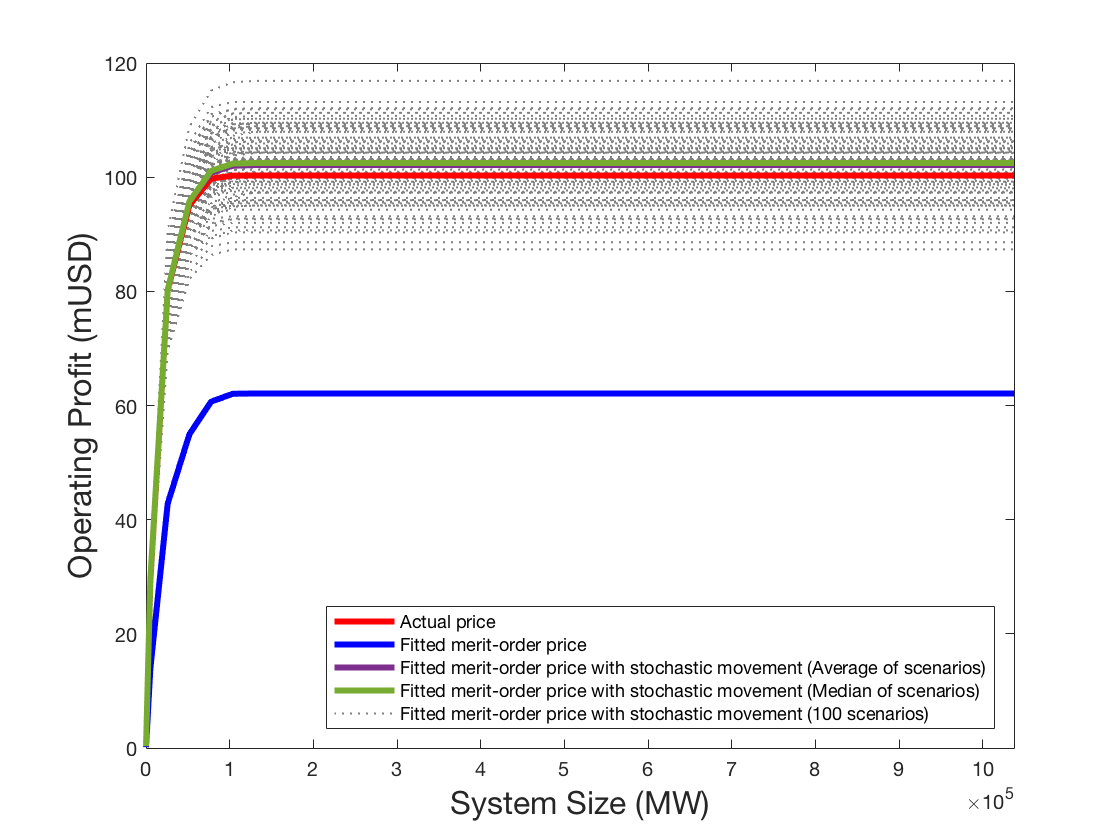
\includegraphics[width=0.95\linewidth]{Figures/6_Model_Validation}
	\caption{The revenue with different price scenarios}
	\label{fig:model-validation}
\end{figure}

\begin{table}[h!]
	\centering
	\begin{tabular}{|r r|}
		\hline
		\multicolumn{2}{|c|}{SARMA parameters}\\
		\hline
		\hline
		$\phi_1 = 1.811$ & $\theta_1 = -1.063$ \\
		$\phi_2 = -0.813$ & $\theta_{24} =0.692$ \\
		$\phi_{24} = 0.090$ & $\theta_{168} = -0.600$ \\
		$\phi_{168} = 0.692$ & \\
		\hline
	\end{tabular}
	\caption{Parameters of the stochastic price movement of SARMA models}\label{tab:SARMA}
\end{table}

Therefore, a seasonal auto-regressed moving-average (SARMA) model as is described in \ref{sec:market-simulation} is applied to simulate the stochastic components of the price. The estimated parameters of the SARMA model based on the error signal characterized by\ref{fig:merit-error} is listed in Table \ref{tab:SARMA}. Thereafter, we conducted Monte-Carlo simulations and generated a number of scenarios of the stochastic parts of price which are then added to the determinate trends calculated by the merit-order model. The final simulated price scenarios are illustrated by the grey lines in Figure \ref{fig:price-example}. Using these generated price profiles, we calculated the revenue for 100 scenarios and compare the average and median value to the result obtained with actual price signal, which shew perfect fitness in Figure \ref{fig:model-validation}. There are no significant differences between the average and median value observed, but for robustness and avoiding effects of outliers, we would use the median value as the simulated result for experiments in proceeding sections.

\subsubsection{Impact of renewable penetration}



\subsubsection{Impact of increasing flexibility}


\subsection{Sensitivity analysis}
\subsubsection{Limited predictability}


\subsubsection{Database}

\subsubsection{Locational price}

\subsubsection{Sensitivity analysis of other parameters}





